\chapter{Approach}
\label{ch:approach}

\instructions{Page budget for Approach: 20-30 pages
%
\begin{itemize}
    \item This chapter describes your main contributions (i.e., what you did) and the decisions that went into them (i.e., why did you did it the way you did it).
    \item Alternative headings may be used depending on the kind of contribution(s) you make.
\end{itemize}
}

\section{Overview}

\instructions{
\begin{itemize}
    \item This section should explain the high-level design
    \item Include possibly an architecture figure that shows how the different parts fit together and what processing/technology/tools/datasets have been used for the different components.
\end{itemize}
%
Name these themes based on the different components or sub-problems you are solving in your thesis.
}

\section{Data Exploration}

For this thesis, exploration of approaches to achieve fairness and interpretability in machine learning algorithms is the goal. The Adult dataset \footnote{https://archive.ics.uci.edu/ml/datasets/adult} was selected for this topic. Before beginning on implementing machine learning methods and experiments, some preliminary data exploration is in order.

\subsection{The Adult Dataset}
\label{sec:adult}
The adult dataset is a dataset extracted by Barry Becker from the 1994 US Census database, and the prediction task is to determine whether a person makes over 50k a year. It consists of the following attributes:

\begin{itemize}
    \item Age: The age of the individual (Positive integer)
    \item Work class: The sector the individual works in (8 Categories)
    \item fnlgwgt: A weight determined by the census bureau (Positive integer)
    \item Education: Highest educational degree (16 categories)
    \item Educaitional-num: Enumerated education (16 categories)
    \item Marital Status: Marital status of individual (7 Categories)
    \item Occupation: General type of occupation (15 categories)
    \item Relationship: What kind of relationship the individual is to others (6 categories)
    \item Race: What race the individual belongs to (6 Categories)
    \item Gender: Biological sex of the individual (2 Categories)
    \item Capital gain: Capital gain of individual (Positive integer)
    \item Capital loss: Capital loss of the individual (Positive integer)
    \item Native country: Native country of the individual (42 categories)
    \item Income: Whether individual makes more than 50K or not (2 Categories)
\end{itemize}

This dataset consists of mostly categorical attributes which are not ordinal. This makes analysis quite challenging. Many models assume Gaussian distributions, which is not present in the dataset. In this dataset, there are also some sensitive attributes, most notably \emph{Gender} and \emph{Race}. One could also argue that \emph{Marital Status} and \emph{Relationship} could also be sensitive attributes.

In a fair machine learning system, we would expect that the outcome in terms of income does not depend on the race, gender, marital status or relationship or the very least that the decision by the model is independent of the sensitive attributes.

\subsection{Attributes correlated with income}

\begin{table}
    \centering
    \begin{tabular}{lr}
        \toprule
        Attribute &  Correlation \\
        \midrule
        marital-status.Never-married &    -0.318782 \\
        relationship.Own-child       &    -0.225691 \\
        relationship.Not-in-family   &    -0.190372 \\
        occupation.Other-service     &    -0.155254 \\
        relationship.Unmarried       &    -0.143642 \\
        education.HS-grad            &    -0.130706 \\
        race.Black                   &    -0.090448 \\
        education.11th               &    -0.086728 \\
        occupation.Adm-clerical      &    -0.086475 \\
        relationship.Other-relative  &    -0.085601 \\
        \bottomrule
    \end{tabular}
    \caption{Features that are negatively correlated with income.}
    \label{fig:negative_income_correaltion}
\end{table}

\begin{table}
    \centering
    \begin{tabular}{lr}
        \toprule
        Attribute &  Correlation \\
        \midrule
        education.Masters                 &     0.174184 \\
        education.Bachelors               &     0.180371 \\
        occupation.Prof-specialty         &     0.188793 \\
        occupation.Exec-managerial        &     0.210938 \\
        gender.Male                       &     0.214628 \\
        capital-gain                      &     0.223013 \\
        hours-per-week                    &     0.227687 \\
        age                               &     0.230369 \\
        marital-status.Married-civ-spouse &     0.445853 \\
        \bottomrule
    \end{tabular}
    \caption{Features that are positively correlated with income.}
    \label{fig:positive_income_correaltion}
\end{table}

We see  in that there are some categories in the following attributes that are correlated with income

\begin{itemize}
    \item Marital Status
    \item Age
    \item Hours per week
    \item Capital Gain
    \item Occupation
    \item Relationship
    \item Education
    \item Gender
    \item Race
\end{itemize}

We observe that our identified sensitive attributes are correlated with income. The challenge now is that we have to learn a model that does not treat individuals belonging to different classes in the sensitive attribute unfairly.

\subsection{Compas Dataset}
The Compas dataset contains records for defendants from Broward County indicating their jail and prison times, demographics, criminal histories and Compas risk scores from 2013 to 2014 \cite{Mehrabi:2021:CSUR}. This dataset is high dimensional with a mix of categorical, numerical and date time columns. For this thesis, the focus has not been to implement the best model out there, but rather compare the fairness between models. Therefore, we have limited ourselves to the following attributes when training our algorithms

\begin{itemize}
    \item Sex: Gender of individual (binary)
    \item Age: Age of individual (positive integer)
    \item Race: Ethnicity of individual (6 categories)
    \item Priors Count: Prior Crimes (positive integer)
    \item Juvenile felony count: Felonies as a juvenile (positive integer)
    \item Juvenile misdemeanour count: Misdemeanours as a juvenile (positive integer)
    \item Juvenile other count: Other charges as a juvenile (positive integer)
    \item Charge degree: Degree of current charge (binary)
    \item Two year recidivism: Whether individual reoffended within two years (binary)
\end{itemize}

We selected these attributes mainly due to these being the only attributes in the dataset that are not recorded after rearrest and were not in a date time format. The point is not to make the best performing classifier, but to compare classifiers with regard to fairness.

\section{Metric for fair machine learning}

Using demographic parity as described in equation~\ref{eq:dempar} is the metric of choice for evaluating the model fairness in this thesis. The main reason for this is that the metric does not assume that the dataset labels are fair. Demographic parity is appropriate to use when we want our predictions to be more in line with a state of nature that we want to see in the world and when we are aware of historical biases that affect the data.~\footnote{\url{https://bit.ly/3Ko10sL}}. In the case of the adult dataset described in section~\ref{sec:adult}, we have the binary sensitive attributes \emph{gender} and the categorical sensitive attribute \emph{race}, both of which are known to experience discrimination in income. 

\begin{figure}
    \centering
    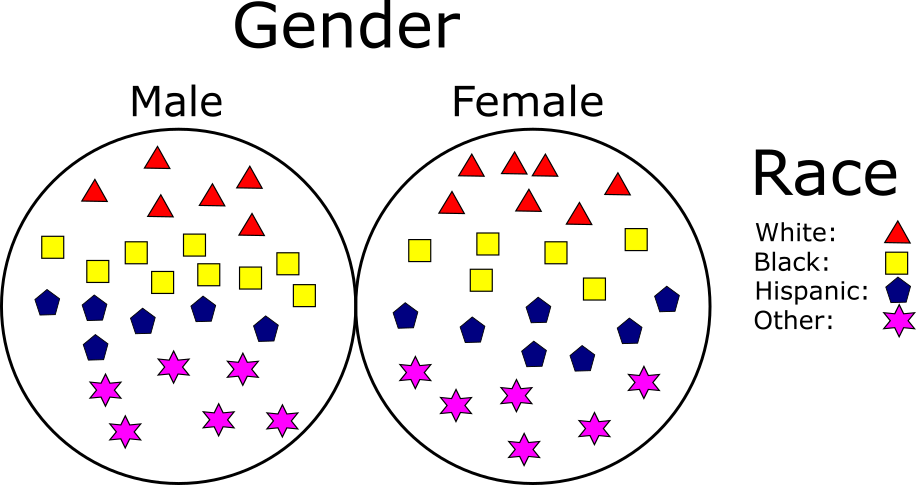
\includegraphics[width=0.7\linewidth]{figures/GroupOverlap.png}
    \caption{Visualisation of overlapping groups.}
    \label{fig:overlap}
\end{figure}

A challenge when working with multiple sensitive attributes and multivariate sensitive attributes is that you get overlapping groups. See figure~\ref{fig:overlap} for an example. There we see that we have the binary attribute \emph{Gender} and the categorical \emph{Race} we have several subgroups, i.e., Black Women, White Male etc. An algorithm can be \emph{independently group fair} when you calculate fairness for each sensitive attribute independently, and/or \emph{intersectional group fair} when you calculate fairness for all subgroups. \cite{Yang:2020:CoRR}. In this thesis, we use both approaches to calculate parity. 

\subsection{Scoring Function: Demographic Parity Score}
\label{sec:demparscore}
We defined anew scoring function based on demographic parity in equation~\ref{eq:dempar}, where $\hat{Y}$ is the predictor and $S$ the sensitive attribute. This equation can be generalised to the case where we have a categorical sensitive attribute with $K$ classes.

$$
P(\hat{Y} | S_i) = P(\hat{Y} | S_j) \qquad i, j \in \{0, \dots, K-1\}, \qquad i \neq j
$$

When calculating the probabilities, we want to condense these probabilities to a single metric between $0$ and $1$. I.e, when we have the likelihood of a positive outcome for the different classes of a sensitive attribute in a list of  probabilities $L$ like so

$$
L =\{ P(\hat{Y}=1 | S=0), \dots, P(\hat{Y}=1 | S=K-1) \}
$$

We want a function $f$ that takes such a list and maps it to a real number between $0$ and $1$

$$
f: L \rightarrow [0, 1]
$$

It is important that this function works for a list of likelihoods of arbitrary length, since we want to evaluate demographic parity for both binary and categorical sensitive attributes as well as all intersections of the sensitive attributes. Given the definition of demographic parity, we want the likelihoods to be as equal as possible. The scoring function derived is shown below

$$
f = 1 - 2\sigma(L)
$$

\begin{table}[]
    \centering
    \begin{tabular}{|l|l|}
        \hline
        $L$                 & $f$  \\ \hline
        {[}0.5, 0.5{]}      & 1    \\ \hline
        {[}0.6, 0.7{]}      & 0.9  \\ \hline
        {[}0.6, 0.8, 0.4{]} & 0.67 \\ \hline
        {[}0, 1, 0, 1{]}    & 0    \\ \hline
    \end{tabular}
    \caption{Example of values of $f$ given different lists of likelihoods.}
    \label{tab:scorefunc}
\end{table}

where $\sigma$ denotes the standard deviation. We plotted the scoring function in figure~\ref{fig:scorefunc}. The scoring function receives a list of two probabilities which slowly diverges from being equal at $0.5$ to the complete opposite, i.e $[0, 1]$. When the probabilities are equal, the score is 0 and if they are very different, the score is 0. See the examples of scores in table~\ref{tab:scorefunc}

\begin{figure}
    \centering
    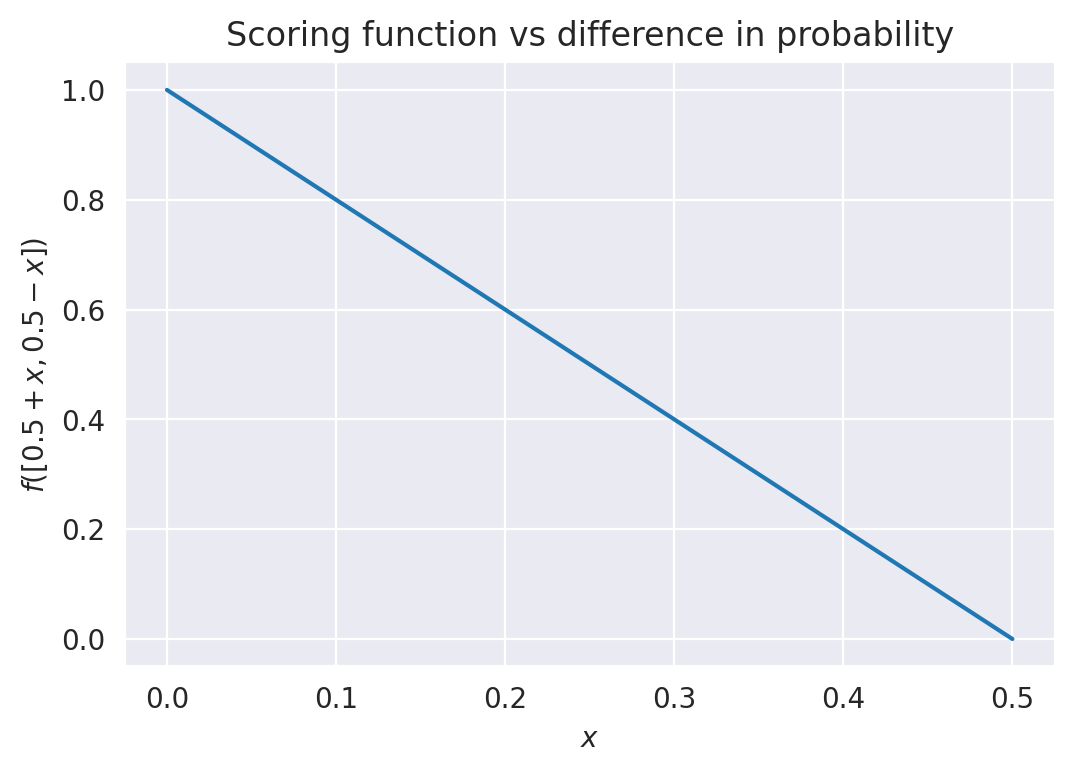
\includegraphics[width=0.7\linewidth]{figures/Parity_metric.png}
    \caption{Scoring function for a list of two diverging probabilities}
    \label{fig:scorefunc}
\end{figure}

\section{Fair Bayesian Network}
\label{sec:fairbayesiannetwork}
Based on the fair Bayesian network described by \citet{Choi:2021:AIII}, the following algorithm was derived.

\begin{algorithm}
    \caption{Latent Label Classifier Training}
    \begin{algorithmic}
        \REQUIRE $D = $ Training Dataset, $S = $ Sensitive Attributes, $L = $ attribute to predict. $t = $ tolerance for expectation maximisation.
        \ENSURE $M = $ Trained Bayesian network.
        \STATE Set of blacklisted nodes: $B = \{(x, y) \quad \forall x \in D.\text{columns}, \quad \forall y \in S\}$
        \STATE $M$.structure $=$ HillClimbSearch($D.$columns $\setminus L$, $B$)
        \STATE $M.$structure$ \cup \{ (x, L) \quad \forall x \in $S$\}$
        \STATE initialise fair node $F$
        \STATE $M.$structure$ \cup \{ (F, x) \quad \forall x \in D.\text{columns}\}$
        \STATE $M.$structure$ \cup \{ (F, L)\}$
        \STATE M.parameters $=$ ExpectationMaximisation($M$.structure, $D$)
        \RETURN M 
    \end{algorithmic}
\end{algorithm}

This method uses two methods implemented in pgmpy \cite{Ankan:2015:SCIPY}. These are Hill Climb Search for learning the structure which is described in section~\ref{HillClimbSearch} and Expectation Maximisation which is described in section~\ref{Expectation Maximization}. The resulting Bayesian network on the adult dataset is shown below in figure~\ref{fig:latentFairClassifierAdult}.

\begin{figure}[h!]
    \centering
    \begin{tikzpicture}[nodes={draw, circle}, ->]
        \node (Race) {$R$};
        \node (Gender) [right=of Race]{$G$};
        \node (Fair) [right=of Gender] {$F$};
        \node (Capital) [below=2cm of Race] {$C$};
        \node (Relationship) [left=of Capital] {$R_e$};
        \node (Education) [left=of Relationship] {$E$};
        \node (Age) [left=of Education] {$A$};
        \node (Marital) [right=of Capital] {$M$};
        \node (Workclass) [right=of Marital] {$W$};
        \node (Hours) [right=of Workclass] {$H$};
        \node (Occupation) [right=of Hours] {$O$};
        \node (Income) [right=of Occupation] {$I$};

        \draw (Fair) -> (Age);
        \draw (Fair) -> (Education);
        \draw (Fair) -> (Relationship);
        \draw (Fair) -> (Capital);
        \draw (Fair) -> (Marital);
        \draw (Fair) -> (Workclass);
        \draw (Fair) -> (Hours);
        \draw (Fair) -> (Occupation);
        \draw (Fair) -> (Income);
        
        \draw (Race) -> (Income);
        \draw (Race) -> (Marital);
        
        \draw (Gender) -> (Relationship);
        \draw (Gender) -> (Marital);
        \draw (Gender) -> (Workclass);
        \draw (Gender) -> (Hours);
        \draw (Gender) -> (Occupation);
        \draw (Gender) -> (Income);
        
        \draw (Age) to  [out=270,in=240] (Hours);
        \draw (Relationship) to  [out=270,in=300] (Age);
        \draw (Relationship) to  [out=270,in=240] (Hours);
        \draw (Marital) to [out=270,in=300] (Age);
        \draw (Marital) to [out=270,in=300] (Relationship);
        \draw (Workclass) to [out=270,in=240] (Occupation);
        \draw (Hours) to [out=270,in=300] (Workclass);
        \draw (Hours) to [out=270,in=240] (Occupation);
        \draw (Occupation) to [out=270, in=300] (Education);
    \end{tikzpicture}
    \caption{latentFairClassifier trained on Adult Dataset. The nodes are $R$: race, $G$: gender, $F$: latent fair labels, $A$: Age, $E$: Education, $R_e$: Relationship, $C$: Capital gain, $M$: Marital Status, $W$: Work class, $H$: Hours-per-week, $O$: Occupation and $I$: Income.}
    \label{fig:latentFairClassifierAdult}
\end{figure}
Inference has been performed by evaluating $P(F | A, E, R_e, C, M, W, H, O)$ on a test dataset of unobserved labels. This is done in pgmpy by using Variable Elimination which is described in section \ref{Variable Elimination}.

\section{Experiment 1: FairBN, FairTreeClassifier vs NB}
\label{sec:AdultFairnessAssessment}

Seven different predictions were evaluated in this experiment. They are the following:

\begin{itemize}
    \item \emph{FairBN}: Training a Fair Bayesian Network and doing inference on the latent fair variable.
    \item  \emph{IncomeBN}: Same model as FairBN. prediction is done on the variable Income instead of the latent fair attribute.
    \item \emph{NBSens} is a naive bayes classifier trained on all of the attributes available. 
    \item \emph{NB} is a naive bayes classifier trained on the dataset without the sensitive attributes. 
    \item \emph{FRFC03}: Fair Random Forest classifier with $\Theta = 0.3$
    \item \emph{FRFC05}: Fair Random Forest classifier with $\Theta = 0.5$
    \item \emph{FRFC07}: Fair Random Forest classifier with $\Theta = 0.7$
\end{itemize} . 

The predictions have been evaluated using the traditional performance metrics \emph{Accuracy}, \emph{Balanced Accuracy}, \emph{F1 Score} and \emph{Specificity}. For fairness, demographic parity score is calculated both independent group fairness and for intersectional group fairness as described in section~\ref{sec:demparscore}. To see the detailed results, these are available in the appendix. See~\ref{app:experiment1}

\begin{figure}
    \centering
    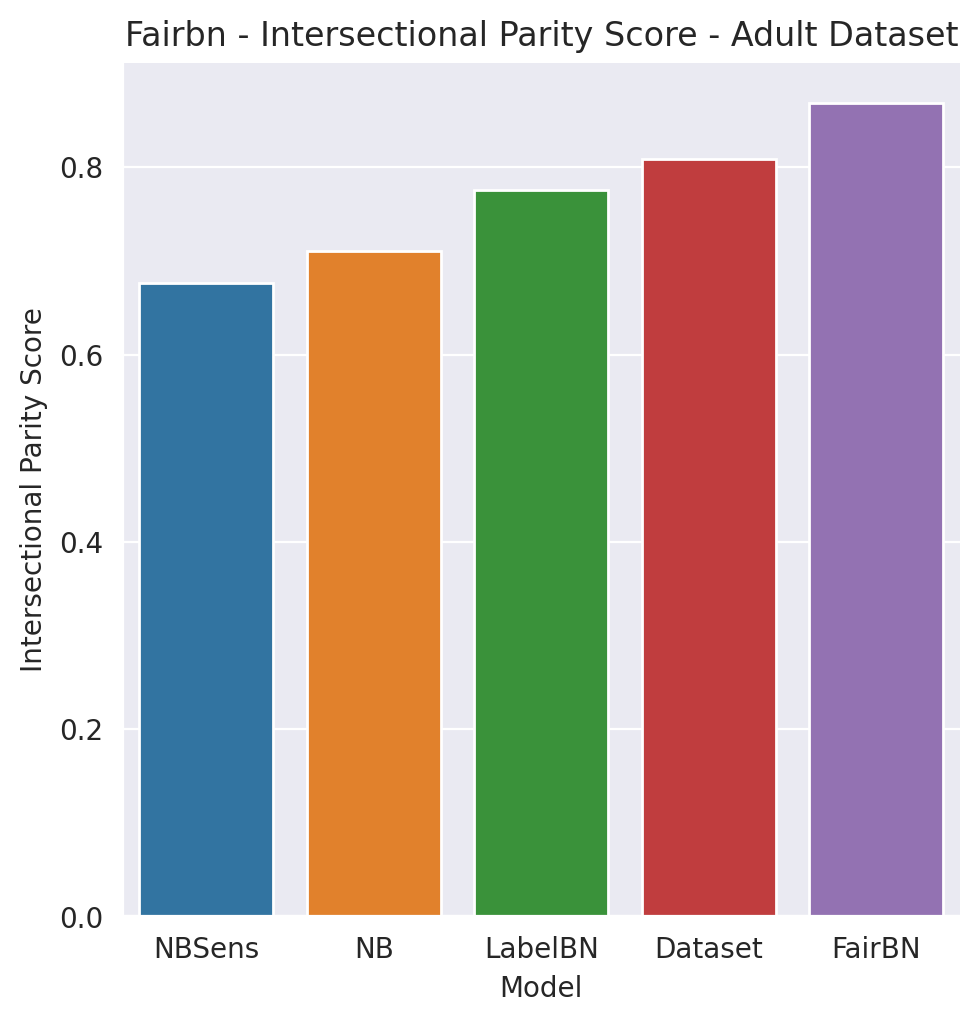
\includegraphics[width=0.49\linewidth]{figures/adult_fairbn_parity.png}
    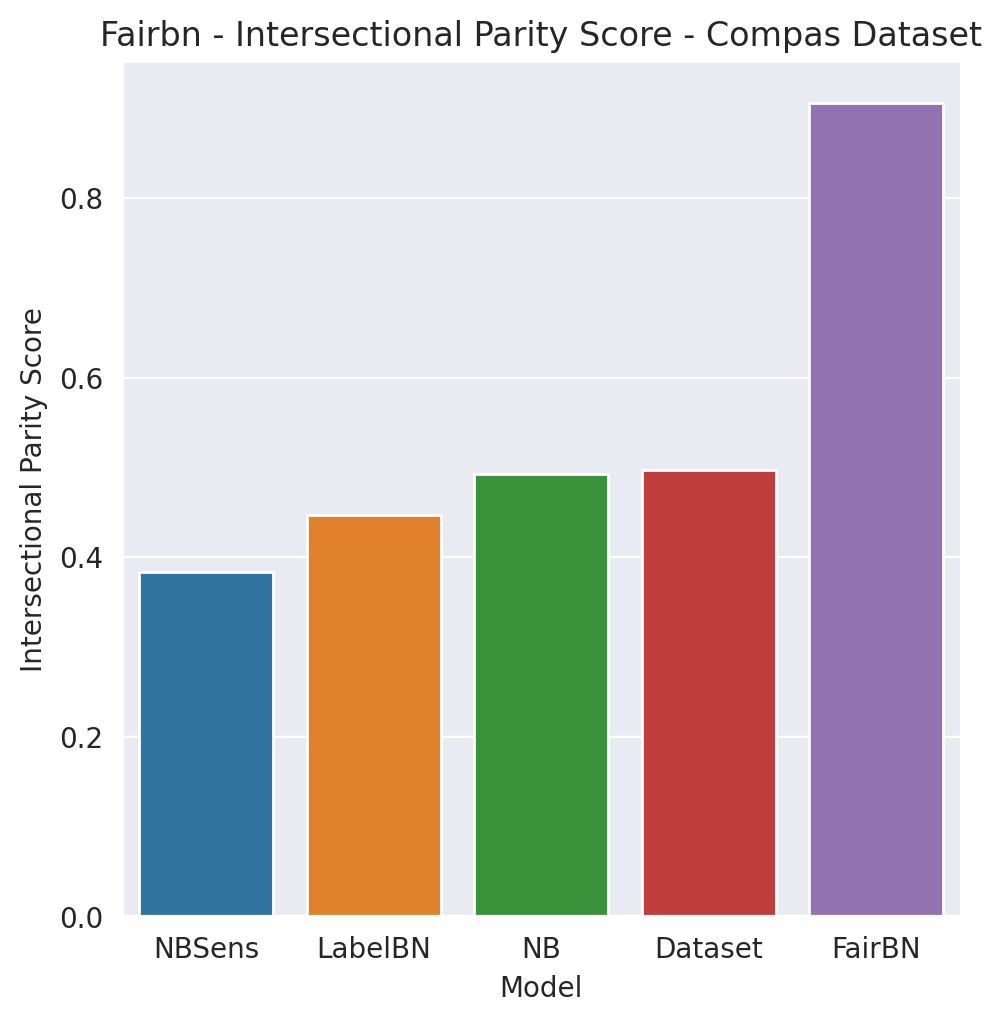
\includegraphics[width=0.49\linewidth]{figures/compas_fairbn_parity.png}
    \caption{Intersectional Parity Score for fair bayesian network vs naive bayes.}
    \label{fig:exp1fairBNparity}
\end{figure}

\subsection{Fair Bayesian Network}

After training the fair bayesian network classifier on the adult and compas dataset, we get an intersectional parity score of $0.87$ and $0.91$ respectively. This is better than the inherent parity score in the dataset labels, which is $0.81$ and $0.51$ respectively. These results and how the different methods compare to one another is shown in figure~\ref{fig:exp1fairBNparity}.

In terms of accuracy and traditional performance of the model, we observe that there is a tradeoff between performance and fairness. This is best shown in the ROC curve shown in figure~\ref{fig:exp1fairBNROC}. There is a slight drop in the fair bayesian network compared to the naive bayes method.

We also observe a quite significant performance difference between the adult dataset and the compas dataset. Why this is is not explored further in this thesis as we are interested in seeing differences in performance with respect to fairness.  
\begin{figure}
    \centering
    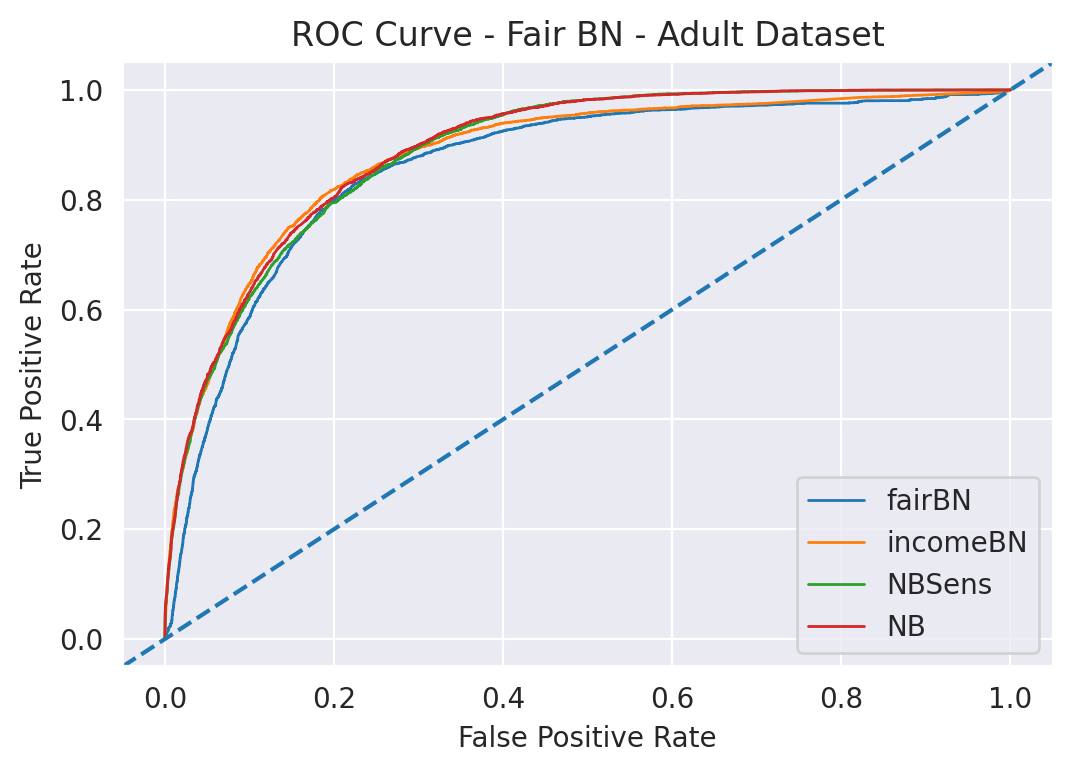
\includegraphics[width=0.49\linewidth]{figures/adult_fairbn_roc.png}
    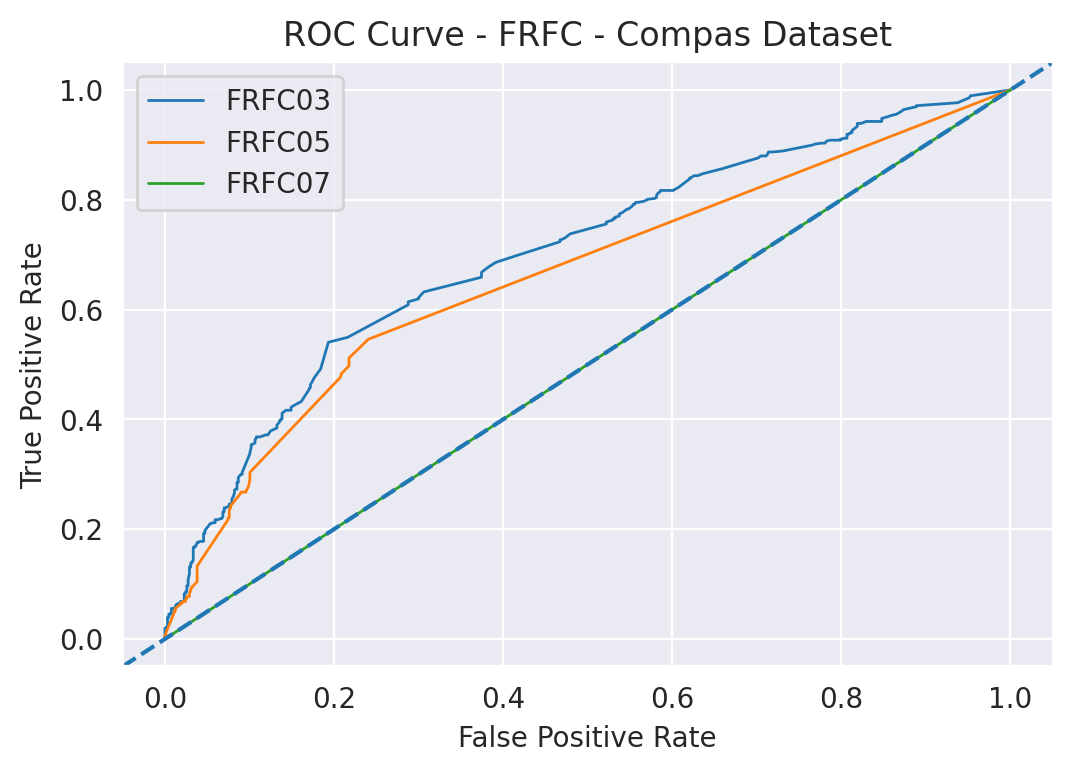
\includegraphics[width=0.49\linewidth]{figures/compas_frfc_roc.png}
    \caption{ROC curve for fair bayesian network vs naive bayes.}
    \label{fig:exp1fairBNROC}
\end{figure}

\subsection{Fair Random Forest Classifier}

\citet{Antonio:2021:arXiv} kindly provided their code on GitHub, which made implementing this over to Forseti a bit easier. The code is available in their repository\footnote{\url{https://bit.ly/3x937Nr}}. We ran the same experiments using their classifier on the adult dataset and compas dataset. Rather interestingly, we do not observe and improvement in intersectional parity in the adult dataset for any of the methods with the inherent intersectional parity for the dataset being $0.810$ and the best fair random forest classifier with $\Theta = 0.3$ having an intersectional parity of $0.78$. Which is counterintuitive to the claimed meaning behind the hyperparameter $\Theta$ stated by the authors.

\begin{figure}
    \centering
    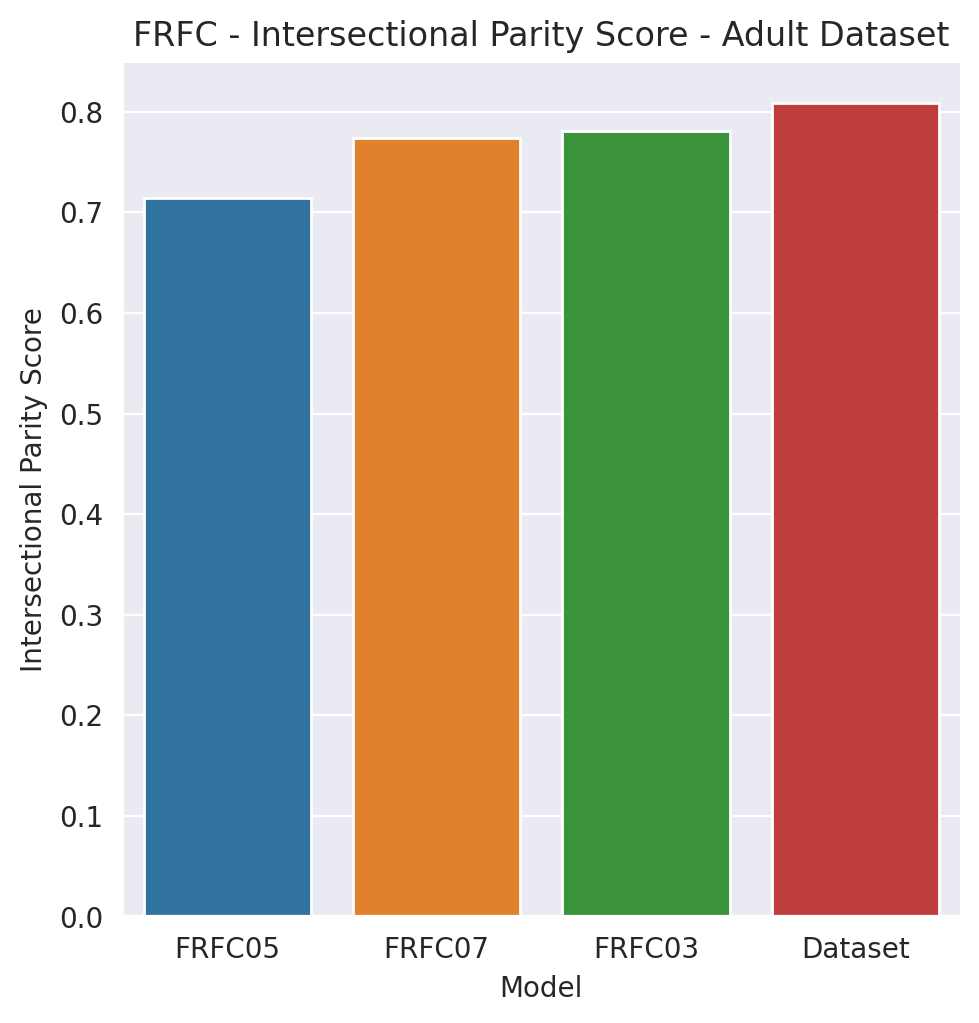
\includegraphics[width=0.49\linewidth]{figures/adult_frfc_parity.png}
    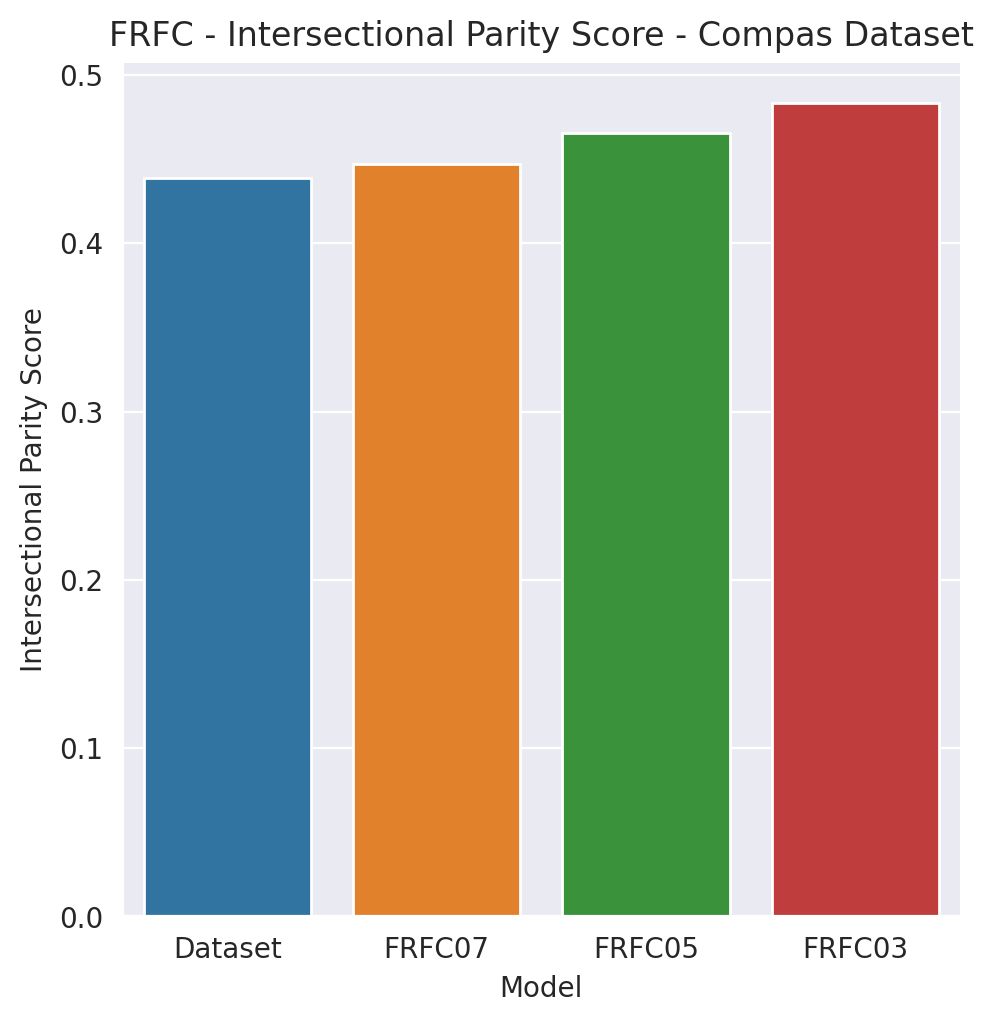
\includegraphics[width=0.49\linewidth]{figures/compas_frfc_parity.png}
    \caption{Parity score for fair random forest classifier.}
    \label{fig:exp1FRFCparity}
\end{figure}

For the Compas dataset, things are looking better with the models with $\Theta \in \{0.3, 0.7\}$ having higher intersectional parity scores than is inherent in the dataset labels. Still, the results given the stated meaning behind $\Theta$ is counterintuitive. The parity scores are shown in figure~\ref{fig:exp1FRFCparity}. The ROC curve for the different datasets is shown in figure~\ref{fig:exp1FRFCROC}

\begin{figure}
    \centering
    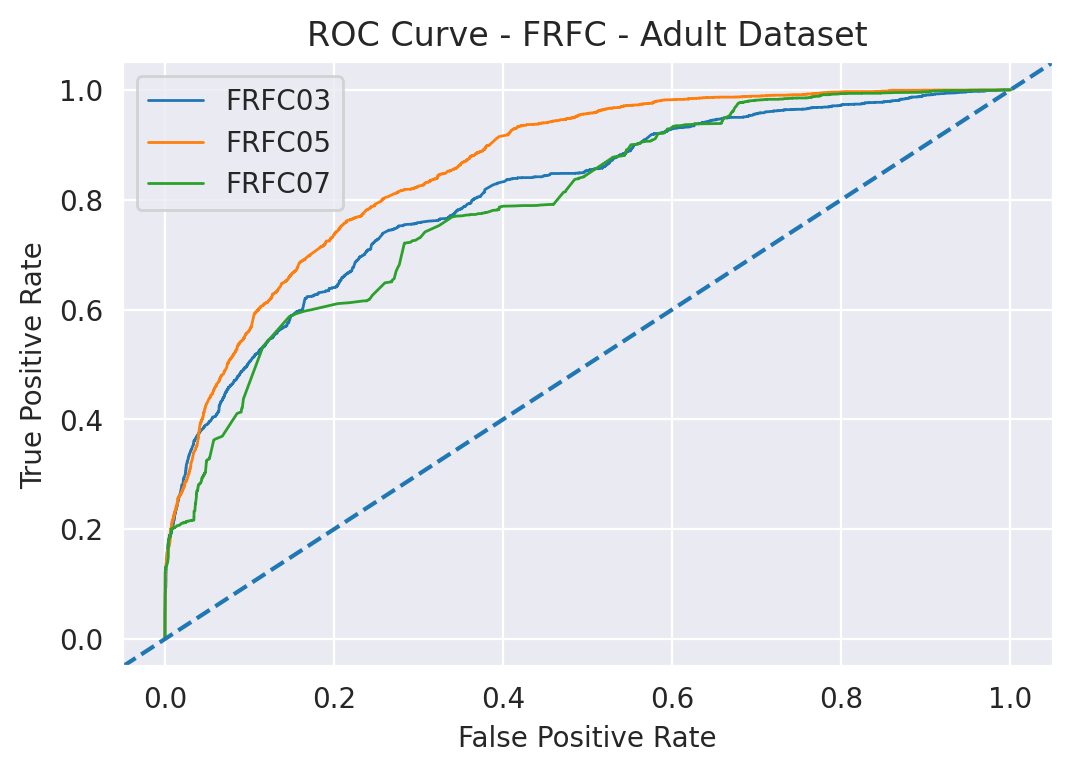
\includegraphics[width=0.49\linewidth]{figures/adult_frfc_roc.png}
    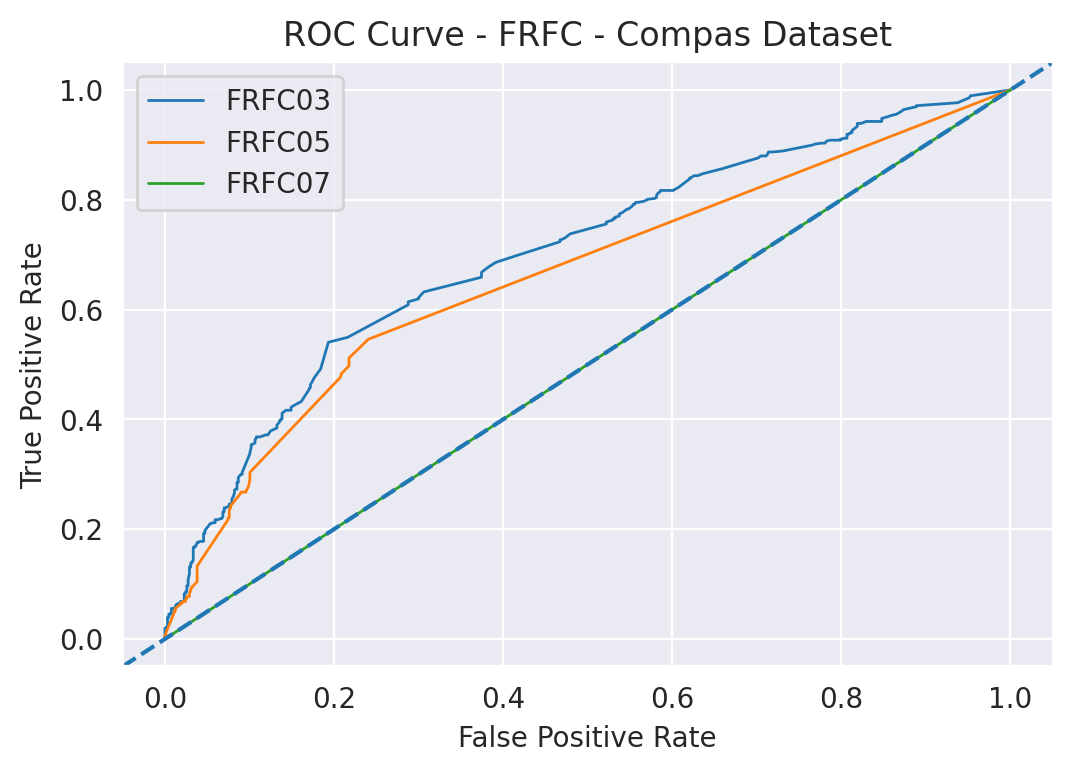
\includegraphics[width=0.49\linewidth]{figures/compas_frfc_roc.png}
    \caption{ROC curve for fair random forest classifier.}
    \label{fig:exp1FRFCROC}
\end{figure}

\subsection{Next experiments}

The results in the first experiment shed some light on the challenge of calculating fairness. The fair bayesian network classifier got higher parity scores as expected but for the random forest classifier, unexplained behaviour of the model with respect to the hyperparameter was observed. Since the parity score used in this experiment is a new and self proposed metric of fairness, this should be investigated further to evaluate its validity.

\citet{Antonio:2021:arXiv} claim that they have made a classifier able to give more fair predictions, and using a hyperparameter $\Theta$ that give more accurate predictions when $\Theta \rightarrow 0$ and more fair predictions when $\Theta \rightarrow 1$. We fail to reproduce these results when calculating parity score for the models. The authors themselves do not calculate intersectional parity score, but rather $AUC_S$ with respect to the individual sensitive attributes.

Due to these observations, we chose to focus on how to calculate fairness and what are the limitations of the respective fairness metrics for the next iteration of experiments.

\section{Experiment 2: Performance on synthetic dataset and comparison of performance metrics.}

The two models that have been implemented in the first round of experiments, namely the fair bayesian network introduced by \citet{Choi:2021:AIII} and the Fair Tree Classifier introduced by \citet{Antonio:2021:arXiv}. These classifiers have two different ways of evaluating fairness that is the motivation behind their design. In the work of \citet{Choi:2021:AIII} the model was designed in terms of demographic parity by modelling a bayesian network in such a way that the sensitive attributes are independent of the predictions but still used for learning the parameters of the distribution of fair labels. In the work of \citet{Antonio:2021:arXiv} they use strong demographic parity as motivation for their model. They implement a tree based method where splits are evaluated using the threshold-independent measure of AUC with respect to the labels of the dataset and  regularised using AUC with respect to the sensitive attributes. 

These methods were compared in the first round of experiments described in section~\ref{sec:AdultFairnessAssessment} the performance of the tree based methods were not as expected. It failed to learn more fair predictions as evaluated by the parity score (see section~\ref{sec:demparscore}). In this experiment, different fairness metrics will be evaluated for both models on synthetic datasets where the amount of unfairness is in our control.

\subsection{Generating Synthetic Data}

We implemented an algorithm for generating synthetic datasets with numerical (Gaussian) features as well as two sensitive features, gender, and race. The dataset can be either informative or non-informative. If the dataset is informative, the features are dependent on the sensitive attributes. I,e there is bias in the data with respect to the sensitive attributes. The dataset is generated the following way. The first attribute, gender $G_s$, is assumed to follow a bernoulli distribution

\begin{equation*}
    G_s \sim B(n, p)
\end{equation*}

where $n = 1$ and $p = 0.5$. I.e. we assume that it is equally likely to be a male or female. The second attribute, Race $R_s$ is assumed to follow a categorical distribution 

\begin{equation*}
    R_s \sim C(k, \boldsymbol{\theta})
\end{equation*}

Which has PMF

\begin{equation*}
    f_{R_s}(R_s = i) = \boldsymbol{\theta}_i, \qquad i \in \{ 1, \dots, k\}
\end{equation*}

where $\boldsymbol{\theta}$ is a vector of $k$ event probabilities $p_i$. $(p_i \geq 0, \sum p_i = 1)$. We want to initilise $\boldsymbol{\theta}$ randomly and this is done by sampling $k$ numbers from $\tau$ wich follows the standard half-normal distribution

\begin{equation*}
    \tau \sim |N(0, 1)|
\end{equation*}

And $\boldsymbol{\theta}$ is then calculated by arranging the $k$ samples from $\tau$ in a vector and transforming them to probabilities 

\begin{equation*}
    \boldsymbol{\theta} = ({\tau_1, \dots, \tau_k}) \cdot \frac{1}{\sum \tau}
\end{equation*}

The numerical values of the sensitive attributes are mapped to strings using a dictionary in python. Now that the sensitive attributes are sampled, we will sample the non-sensitive features. To simulate the discrimination process, we sample the features from Gaussian distributions that depend on the sensitive attributes. There are 4 numerical features where the first two depend on the gender and the last two depend on the race. Let's denote these features $X_1, X_2, X_3$ and $X_4$.

\begin{figure}
    \centering
    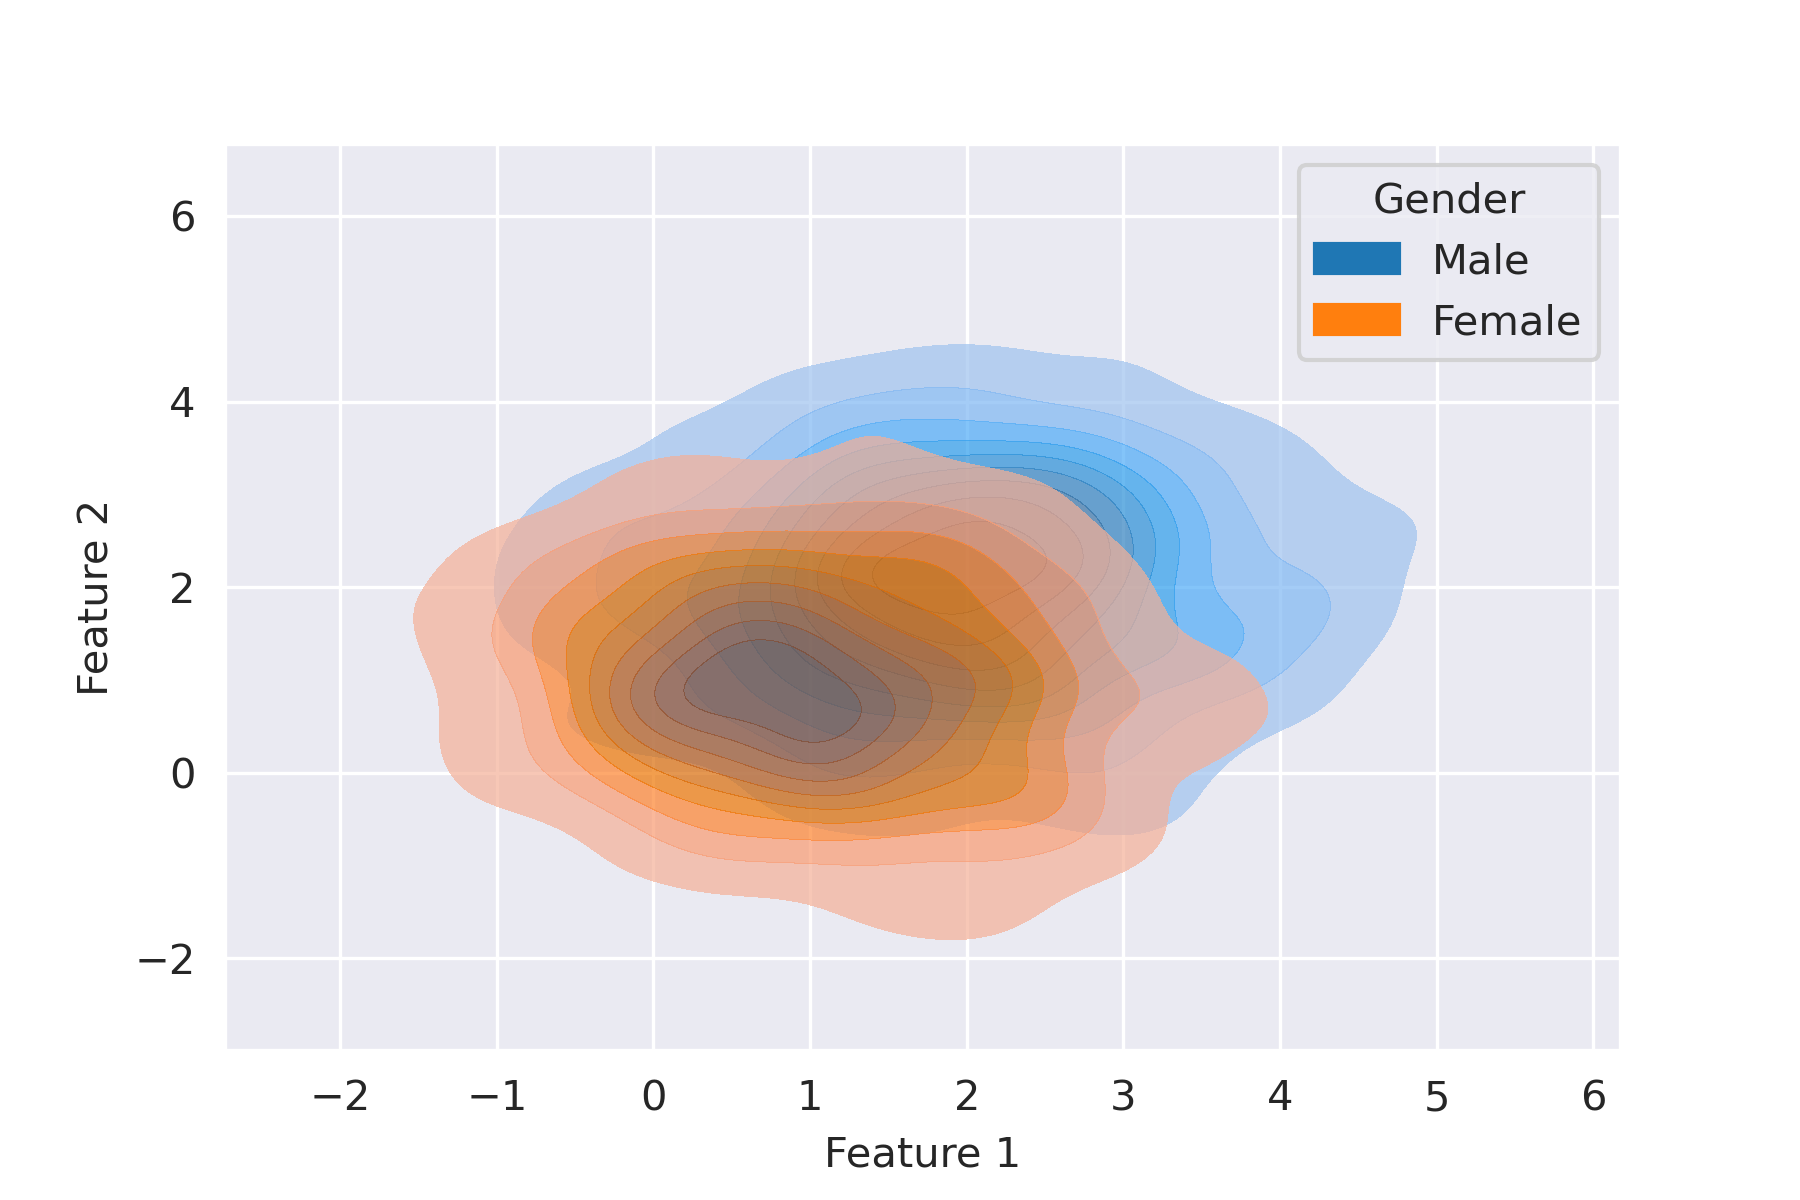
\includegraphics[width=0.49\linewidth]{figures/synthetic-gender.png}
    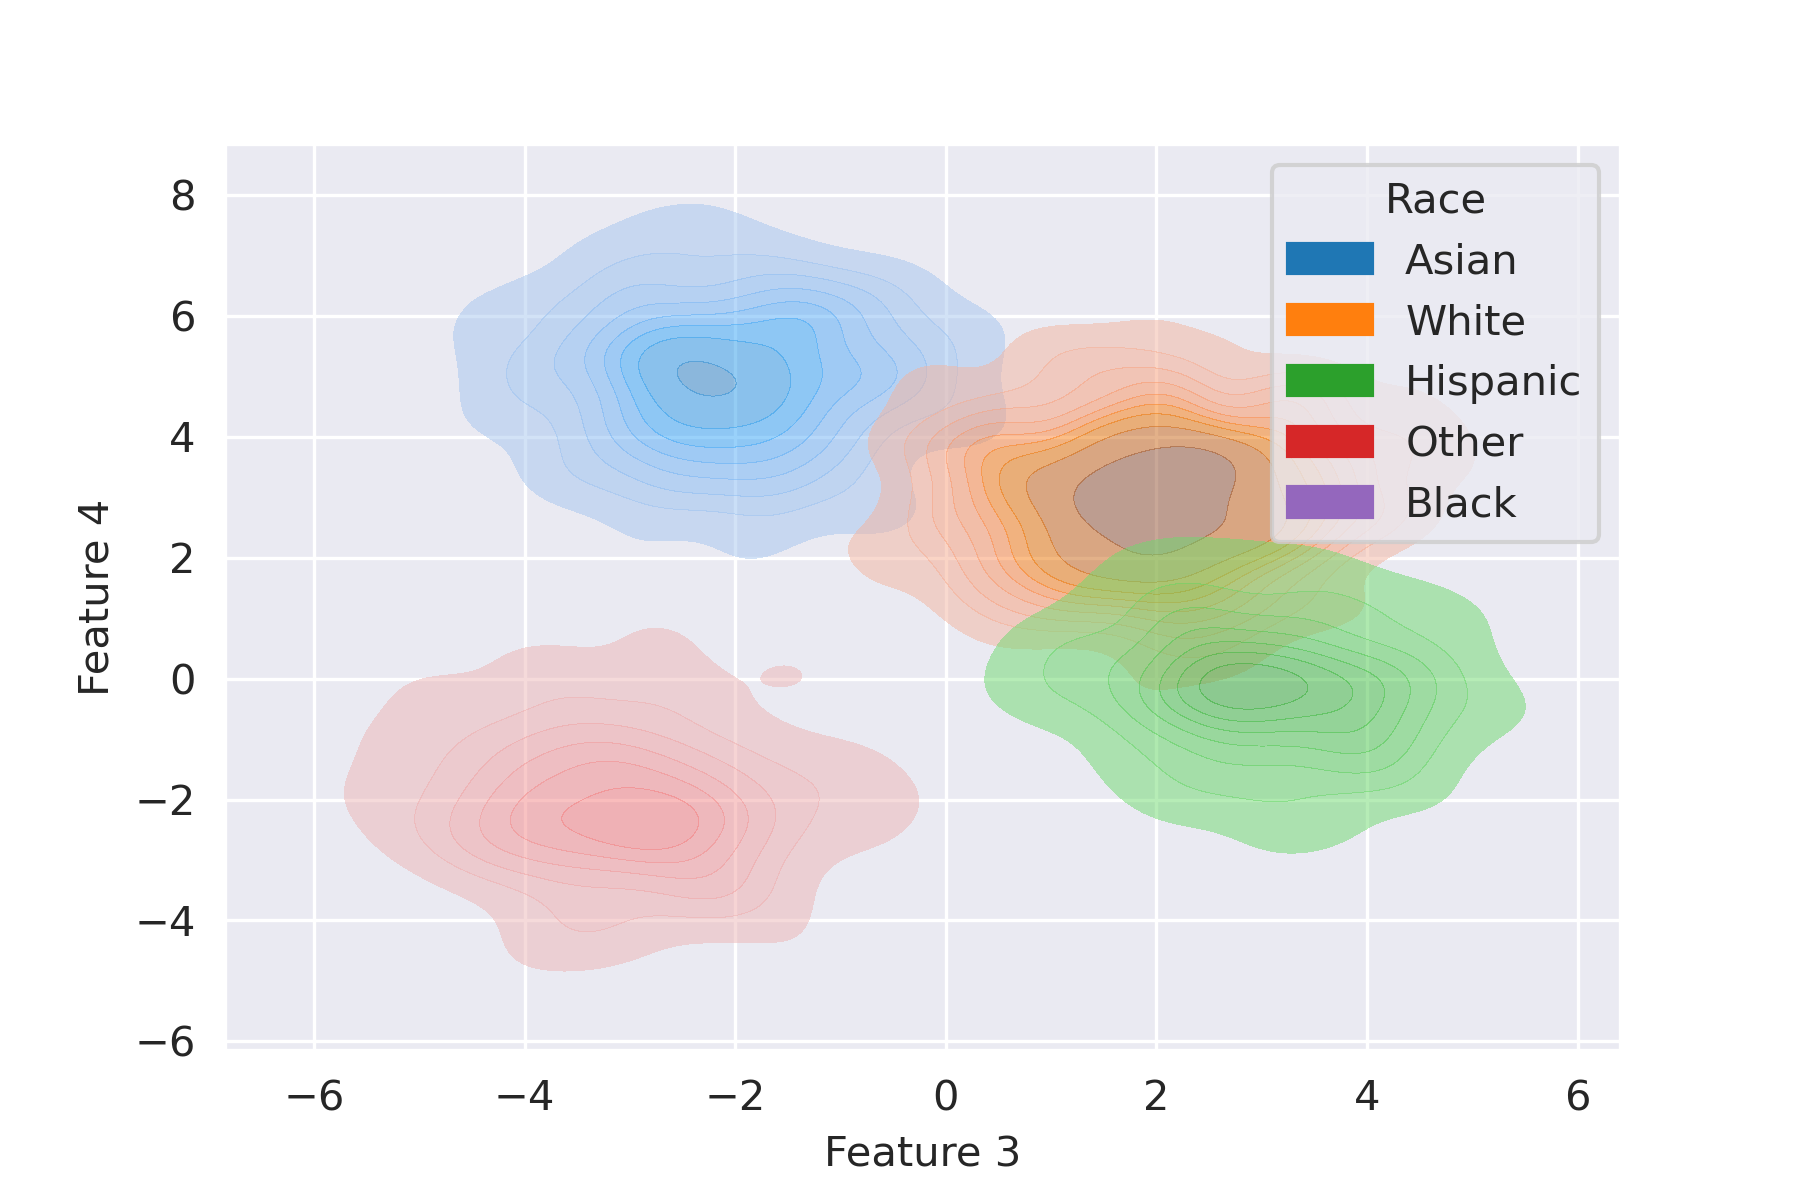
\includegraphics[width=0.49\linewidth]{figures/synthetic-race.png}
    \caption{KDE of the bivariate features of the synthetic dataset..}
    \label{fig:synthdatasetfeatures}
\end{figure}


We define a separator parameter $\Theta$ which is used to model the seperation between the sensitive classes. We sample $X_1$ and $X_2$ the following way conditionally on the sensitive attribute $G_s$

\begin{equation*}
    \begin{aligned}
           X_1 | G_s = \text{Female} \sim N(1, 1) \\ 
           X_1 | G_s = \text{Male} \sim N(1 + \Theta, 1)
    \end{aligned}
\end{equation*}

And the same for $X_2$. The same principle is used for $X_3$ and $X_4$ but with a slight twist. There are $k$ races in the dataset and a random sign variable $R$ following the discrete uniform distribution over the set $\{-1, 1\}$.

\begin{equation*}
    \begin{aligned}
        X_3 | R_s = k \sim N(1 + \Theta \cdot R \cdot k, 1)
    \end{aligned}
\end{equation*}

and the same for $X_4$. Then lastly, to calculate the labels of the dataset we take the sum of all the numerical features $X = \{ X_1, X_2, X_3, X_4 \}$ and calculate the median of all the sums for each datapoint. If the sum is above the median, it gets labeled 1, otherwise, 0.

This can be summarised in algorithm~\ref{alg:datasetgen}

\begin{algorithm}
    \caption{Synthetic dataset generation}
    \begin{algorithmic}
        \REQUIRE $I = $ Informative. True or false, $\Theta = $ Separability, $N =$ Number of samples.
        \ENSURE $D = $ Synthetic Dataset.
        \STATE Sample $N$ samples from $G_s \sim B(1, 0.5)$
        \STATE $k = 5$
        \STATE $\boldsymbol{\tau_k} = \{ \tau_1, \dots, \tau_k \}$ with $\tau_j \sim |N(0, 1)|$
        \STATE $\theta = \boldsymbol{\tau} \cdot \frac{1}{\sum \tau_k}$
        \STATE Sample $N$ samples from $R_s \sim C(k, \theta)$
        \STATE Sample $N_{\text{Female}}$ samples from $X_1 \sim N(1, 1)$
        \STATE Sample $N_{\text{Male}}$ samples from $X_1 \sim N(1 + \Theta, 1)$
        \STATE Sample $N_{\text{Female}}$ samples from $X_2 \sim N(1, 1)$
        \STATE Sample $N_{\text{Male}}$ samples from $X_2 \sim N(1 + \Theta, 1)$
        \FORALL{$i \in \{ 1, \dots, k \}$}
        \STATE Select $R$ uniformly from the set $\{ -1, 1\}$
        \STATE Sample $N_i$ samples from $X_3 | R_s = i \sim N(1 + \Theta \cdot R \cdot i, 1)$
        \STATE Select $R$ uniformly from the set $\{ -1, 1\}$
        \STATE Sample $N_i$ samples from $X_4 | R_s = i \sim N(1 + \Theta \cdot R \cdot i, 1)$
        \ENDFOR
        \STATE $t = \sum X$ for all datapoints in the dataset
        \IF{$t \geq \text{Median}(X)$}
        \STATE $Y = 1$
        \ELSE
        \STATE $Y = 0$
        \ENDIF
        \STATE $D = \{G_s, R_s, X_1, X_2, X_3, X_4, Y \}$
        \RETURN $D$
    \end{algorithmic}
    \label{alg:datasetgen}
\end{algorithm}

\subsection{Fairness Performance Measure}

The performance metric used for the models up to this points it the parity score metric as described in Section.~\ref{sec:demparscore}. This score is based on the notion that the likelihood of positive outcome is independent of the sensitive attributes. There is another measure that is similar to this. That is Kullback-Leibler divergence. Which according to \citet{Mackay:2003:information} is calculated as 

\begin{equation*}
    D_KL(P ||Q) = \sum_x \log\frac{P(x)}{Q(x)}
\end{equation*}

Kullback-Leibler divergence is a measure of how different two distributions $P$ and $Q$ are. It is not strictly a metric as it is not symmetric and is instead a divergence. While metrics are symmetric and linear in distance, divergences are asymmetric and generalise square distance. For our work, we want to use Kullback-Leibler divergence as a measure of unfairness. The general idea is that we want $P$ and $Q$ to denote different distributions conditional on sensitive attributes. Assume that we have a dataset with model predictions $Y$ and a binary sensitive attribute $S$. Then we define 

\begin{equation*}
    P \sim Y | S = 0
\end{equation*}

and

\begin{equation*}
    Q \sim Y | S = 1
\end{equation*}

Under demographic parity, we want $Q \perp\!\!\!\perp P , S$ and thus a Kullback-Leibler Divergence of 0. Kullback-Leibler Divergence is limited to two distributions though there are generalisations. For this round of experiments we limit ourselves to the binary case and calculate the divergence in the binary cases and compare them to the other metrics.

\subsection{Estimating Model Performance}

In the second round of experiments, we want to estimate the model performance distributions. To do this, we ran 100 synthetic dataset generations and trained models on the synthetic datasets and evaluate them on a test dataset. For each iteration the train-test split is $70\%$ for the training set and $30\%$ for the test dataset. In this section the different results are presented.

\subsubsection{F1 Score}

\begin{figure}
    \centering
    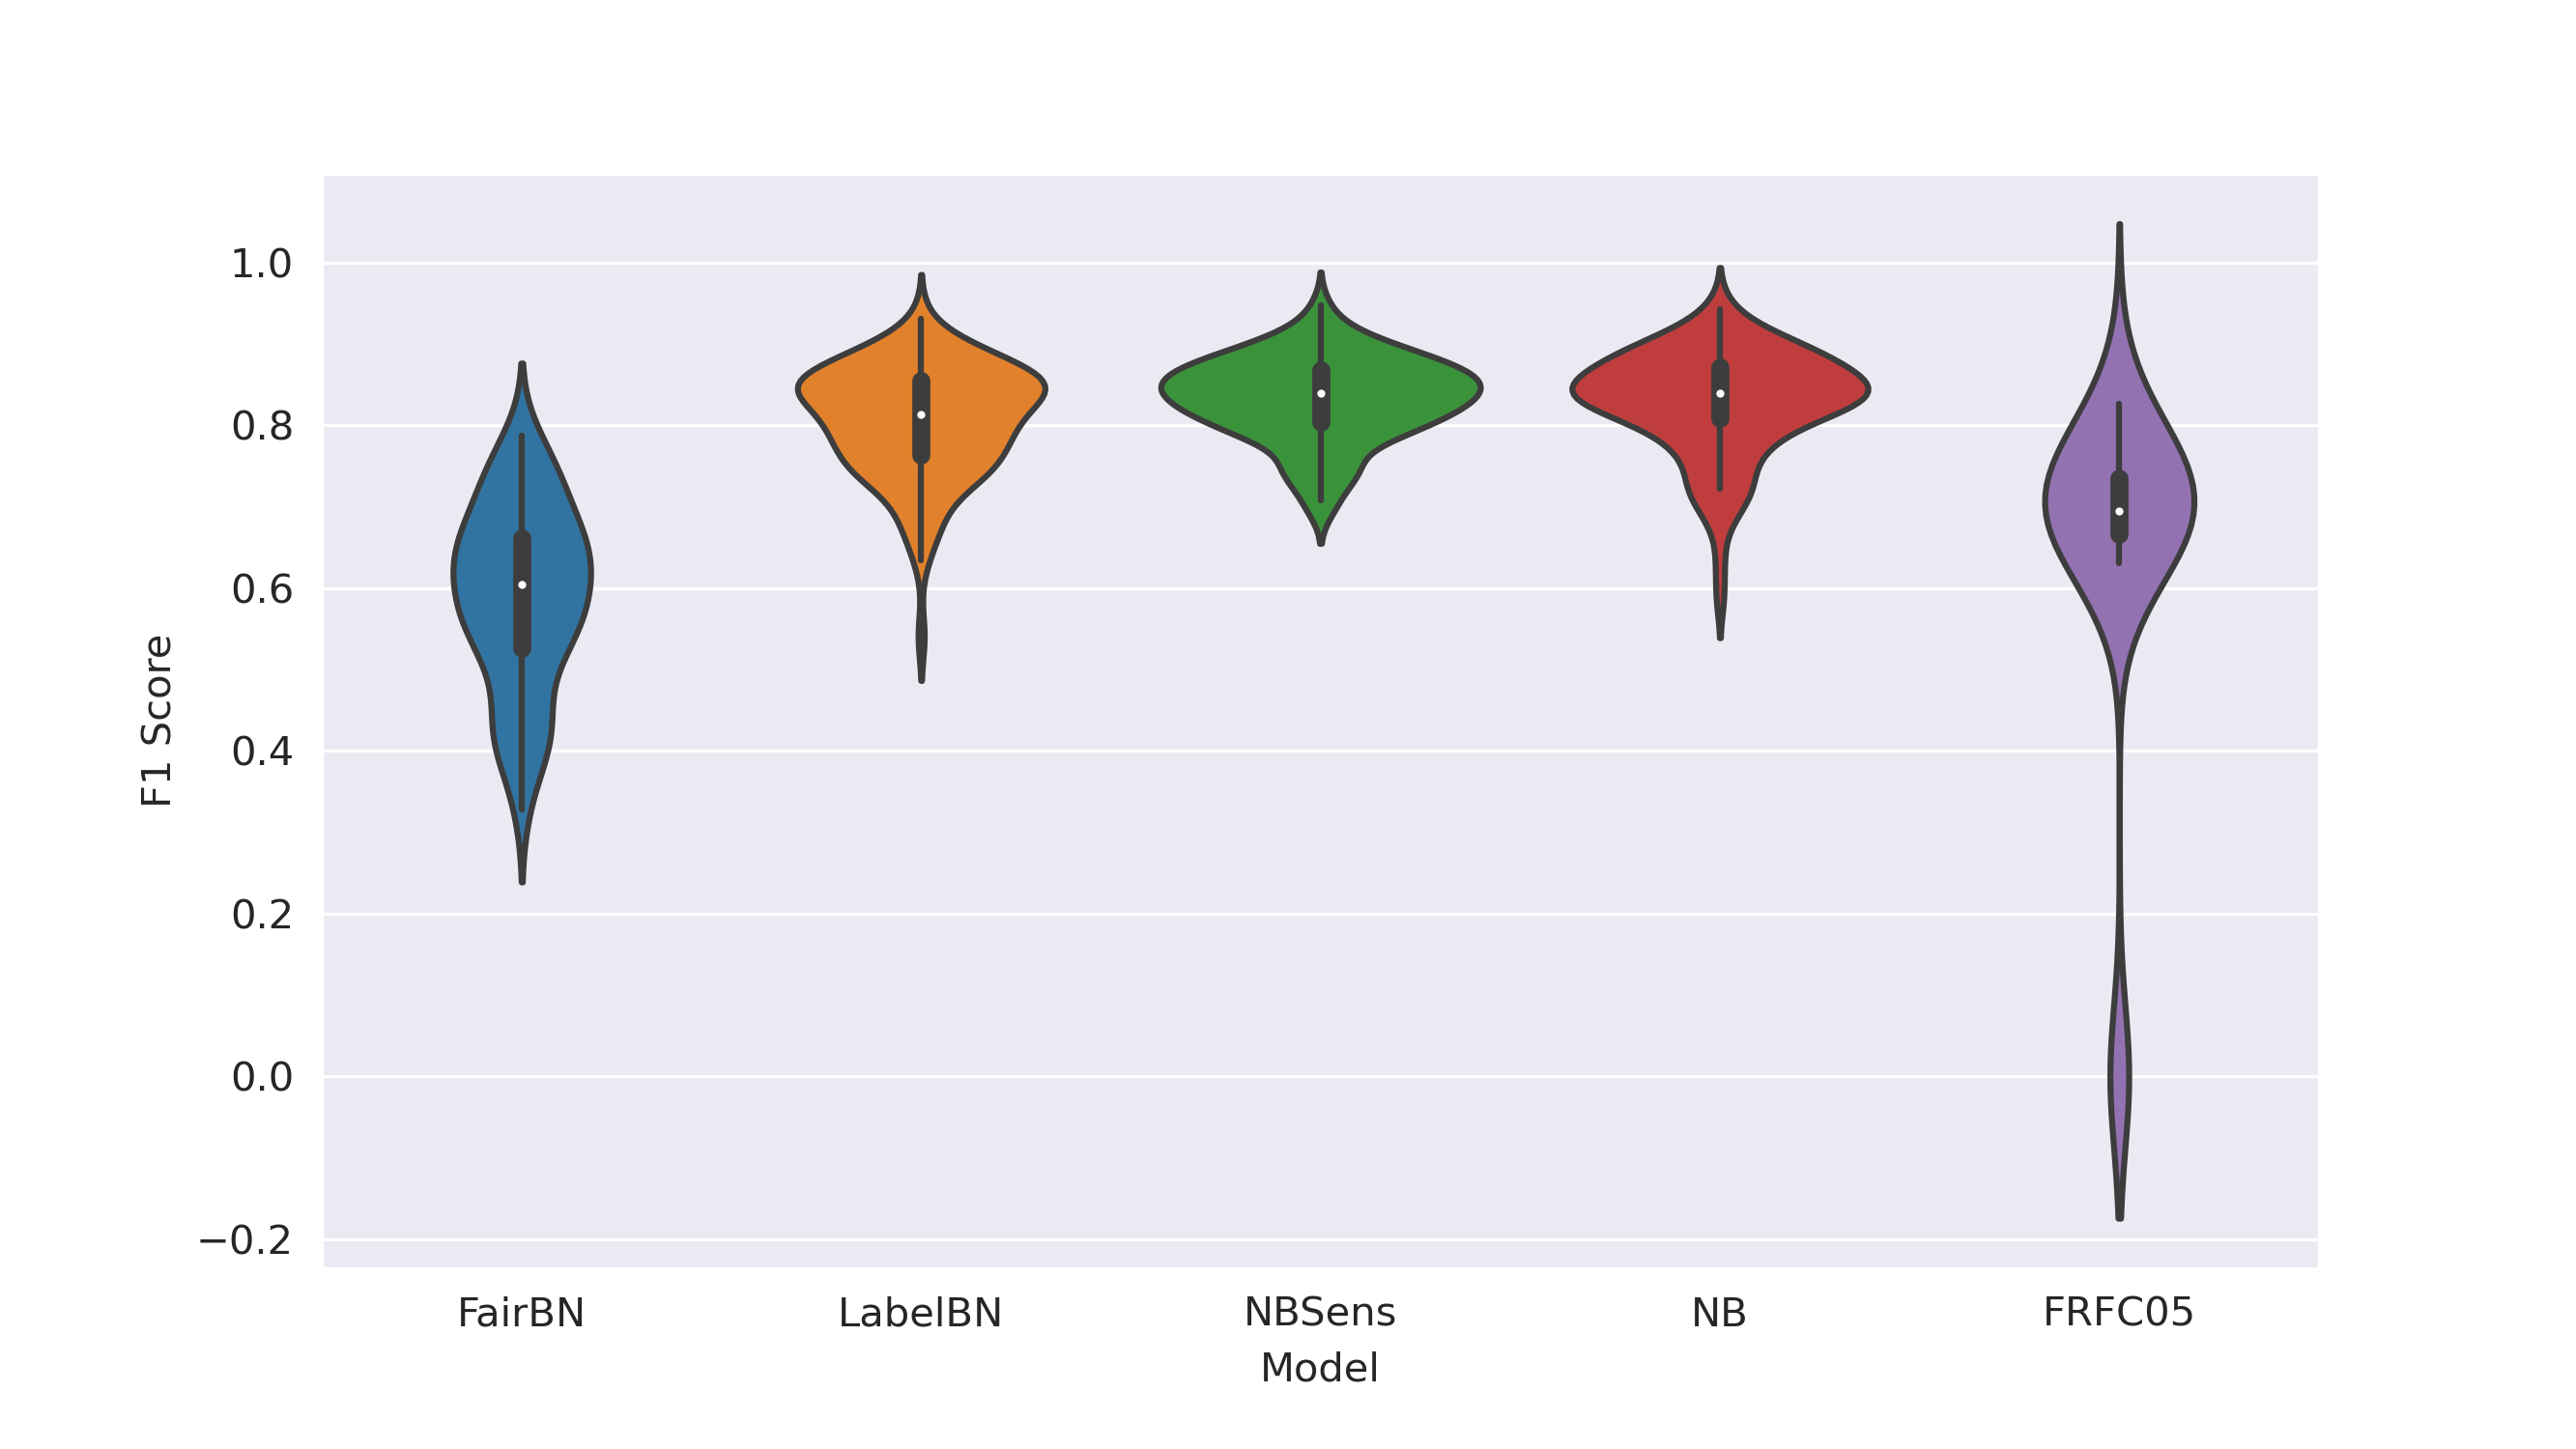
\includegraphics[width=\linewidth]{figures/F1score-synthethic.png}
    \caption{F1 Scores of the different models on 100 synthetic datasets. Higher is better.}
    \label{fig:f1synth}
\end{figure}

When evaluating the models in terms of F1 Score, we observe that the fair methods have lower but acceptable F1 Scores. For the fair bayesian network classifier $95\%$ of the F1 scores is at $0.4$ or higher with mean at $0.6$. For the fair random forest classifier, these values are $0.0$ and $0.63$. We see from the plot in figure~\ref{fig:f1synt} that the F1 score of the fair bayesian network is on average lower than for fair random forest classifier but with lower variance.

\subsubsection{Specificity}

\begin{figure}
    \centering
    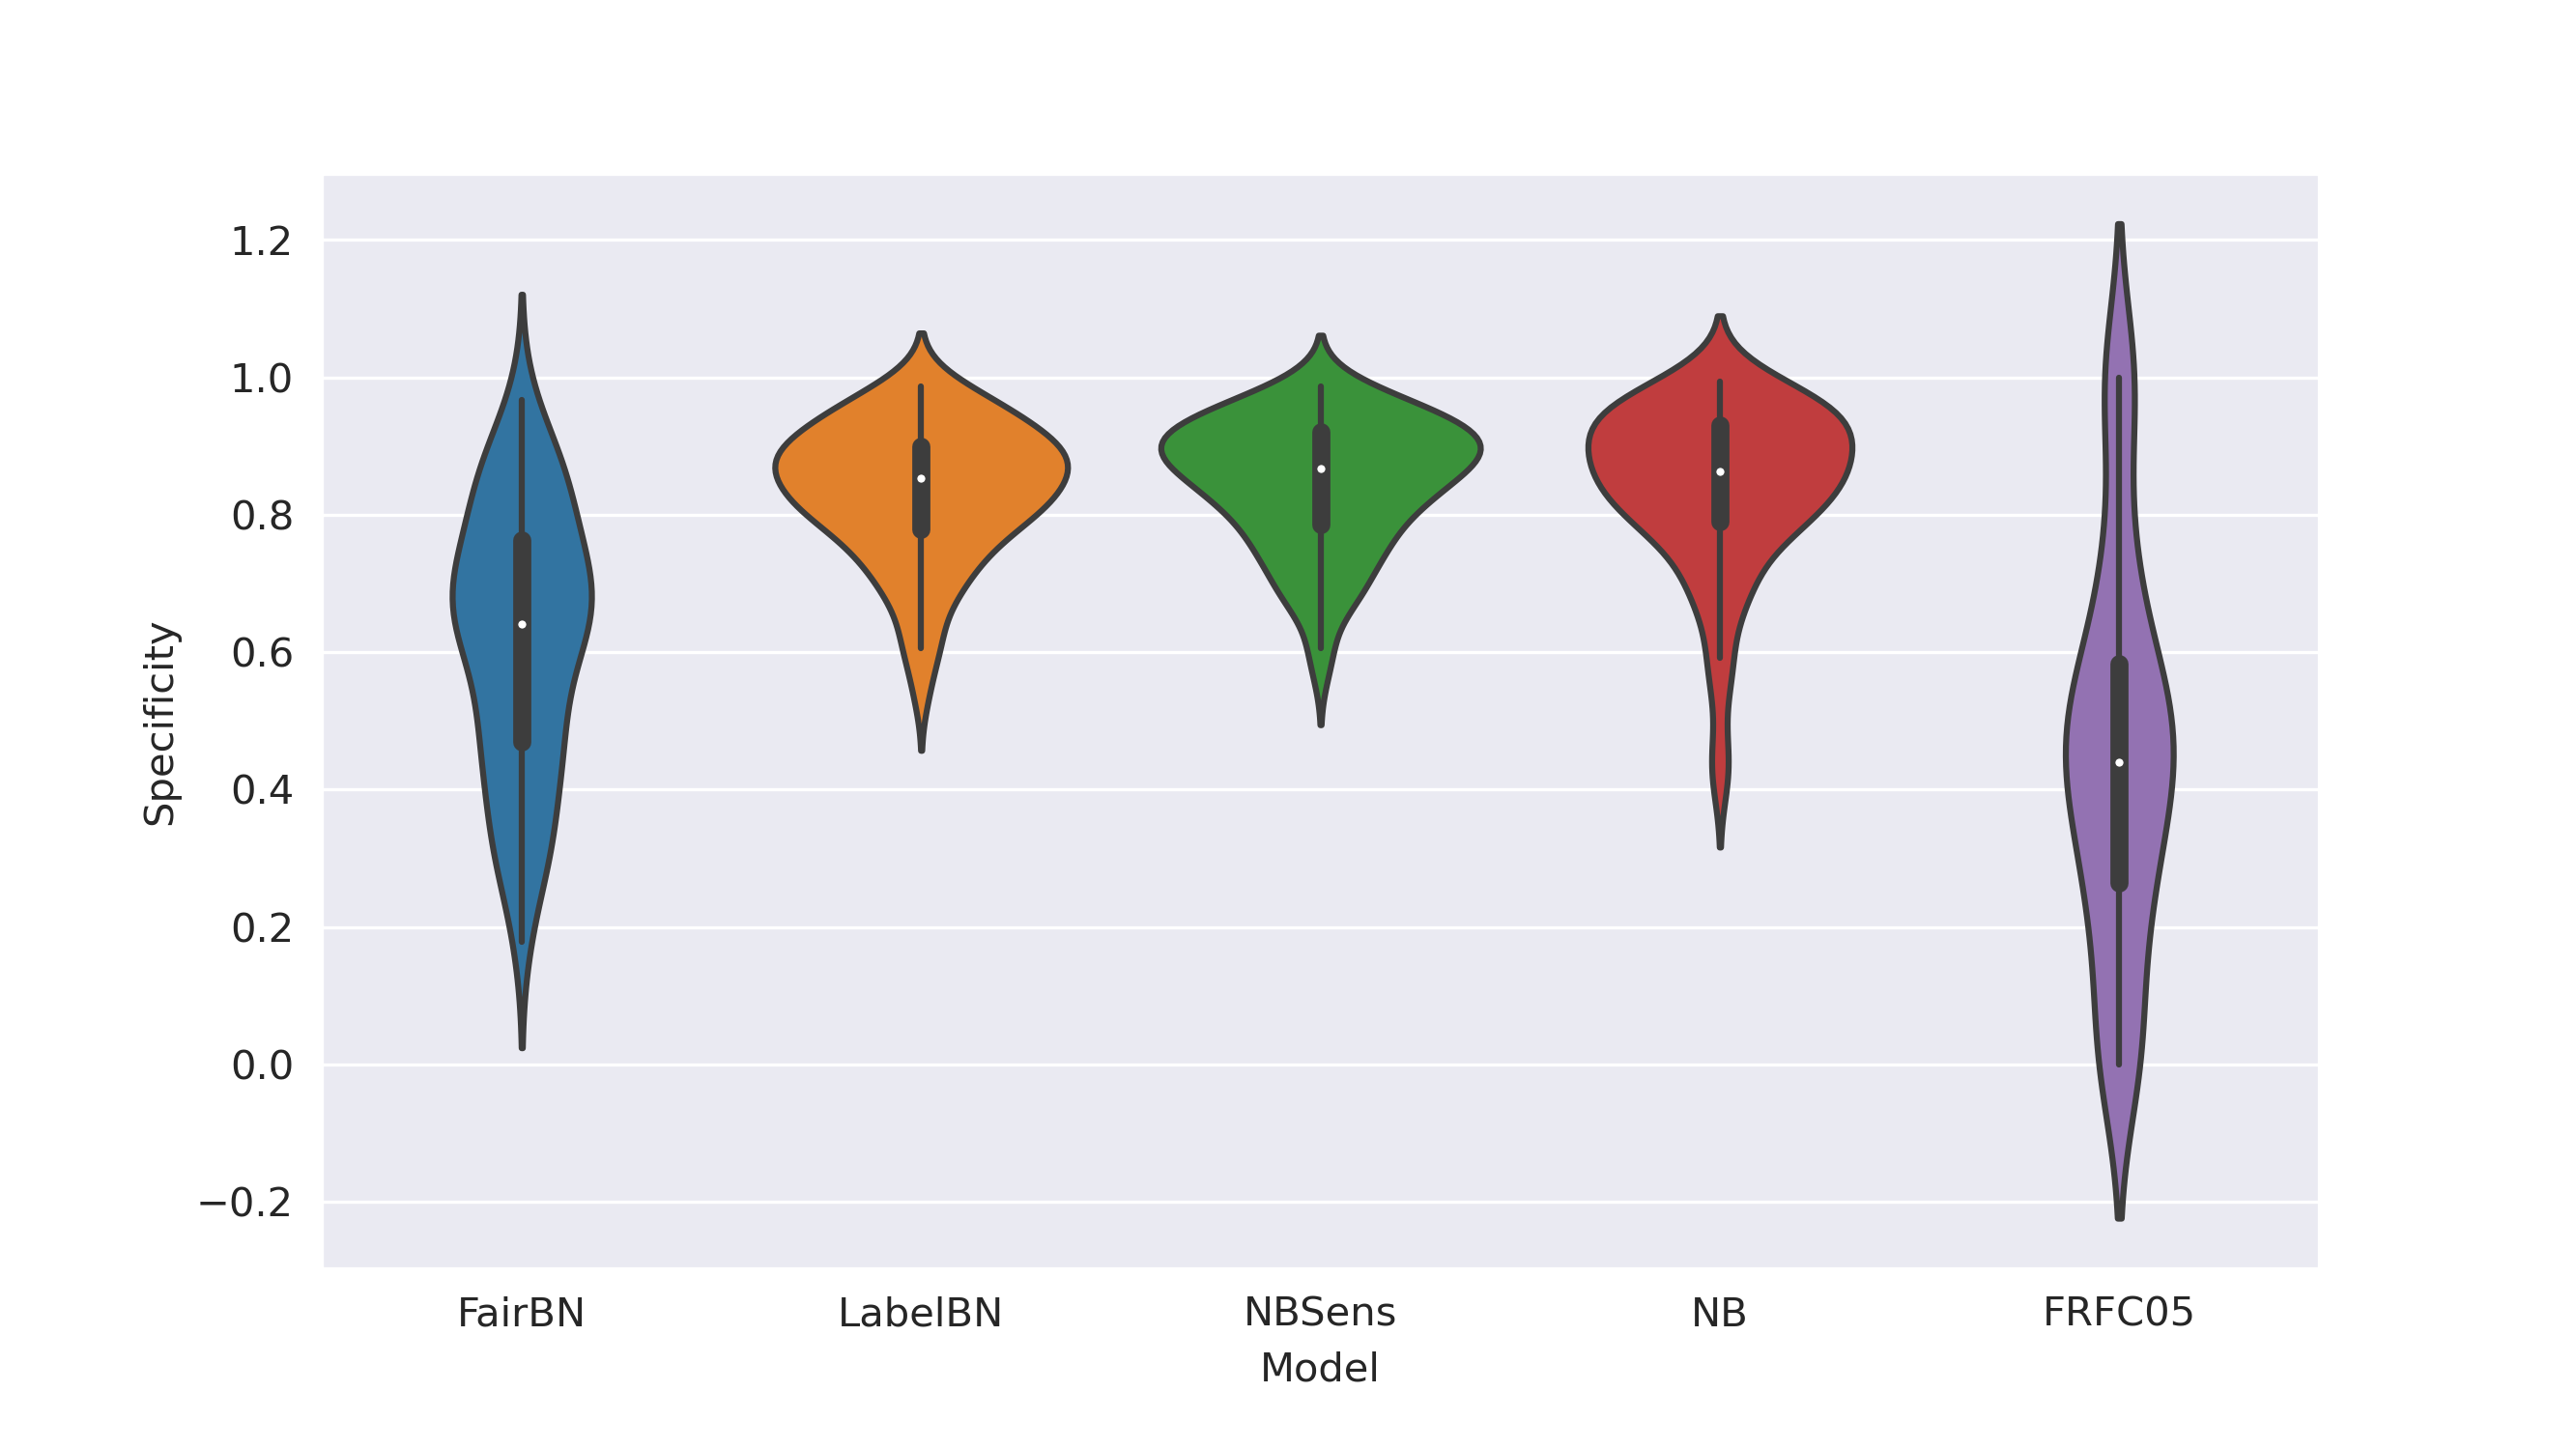
\includegraphics[width=\linewidth]{figures/Specificity-synthetic.png}
    \caption{Specificity of the different models on 100 synthetic datasets. Higher is better}
    \label{fig:specsynth}
\end{figure}

Since F1 Score is biased with respect to true negatives, we calculate the Specificity of the models as well. The distribution of specificity for the different models are shown in figure~\ref{fig:specsynth}. We observe that the fair methods has a higher variance in their specificity as compared to the Naive Bayesian methods as well as the unfair predictions of the fair bayesian network. $95\%$ of the specificity values are at $0.3$ or higher with mean at $0.61$. For fair random forest classifier, these values are $0.0$ and $0.44$ respectively.

\subsubsection{Intersectional parity score}

\begin{figure}
    \centering
    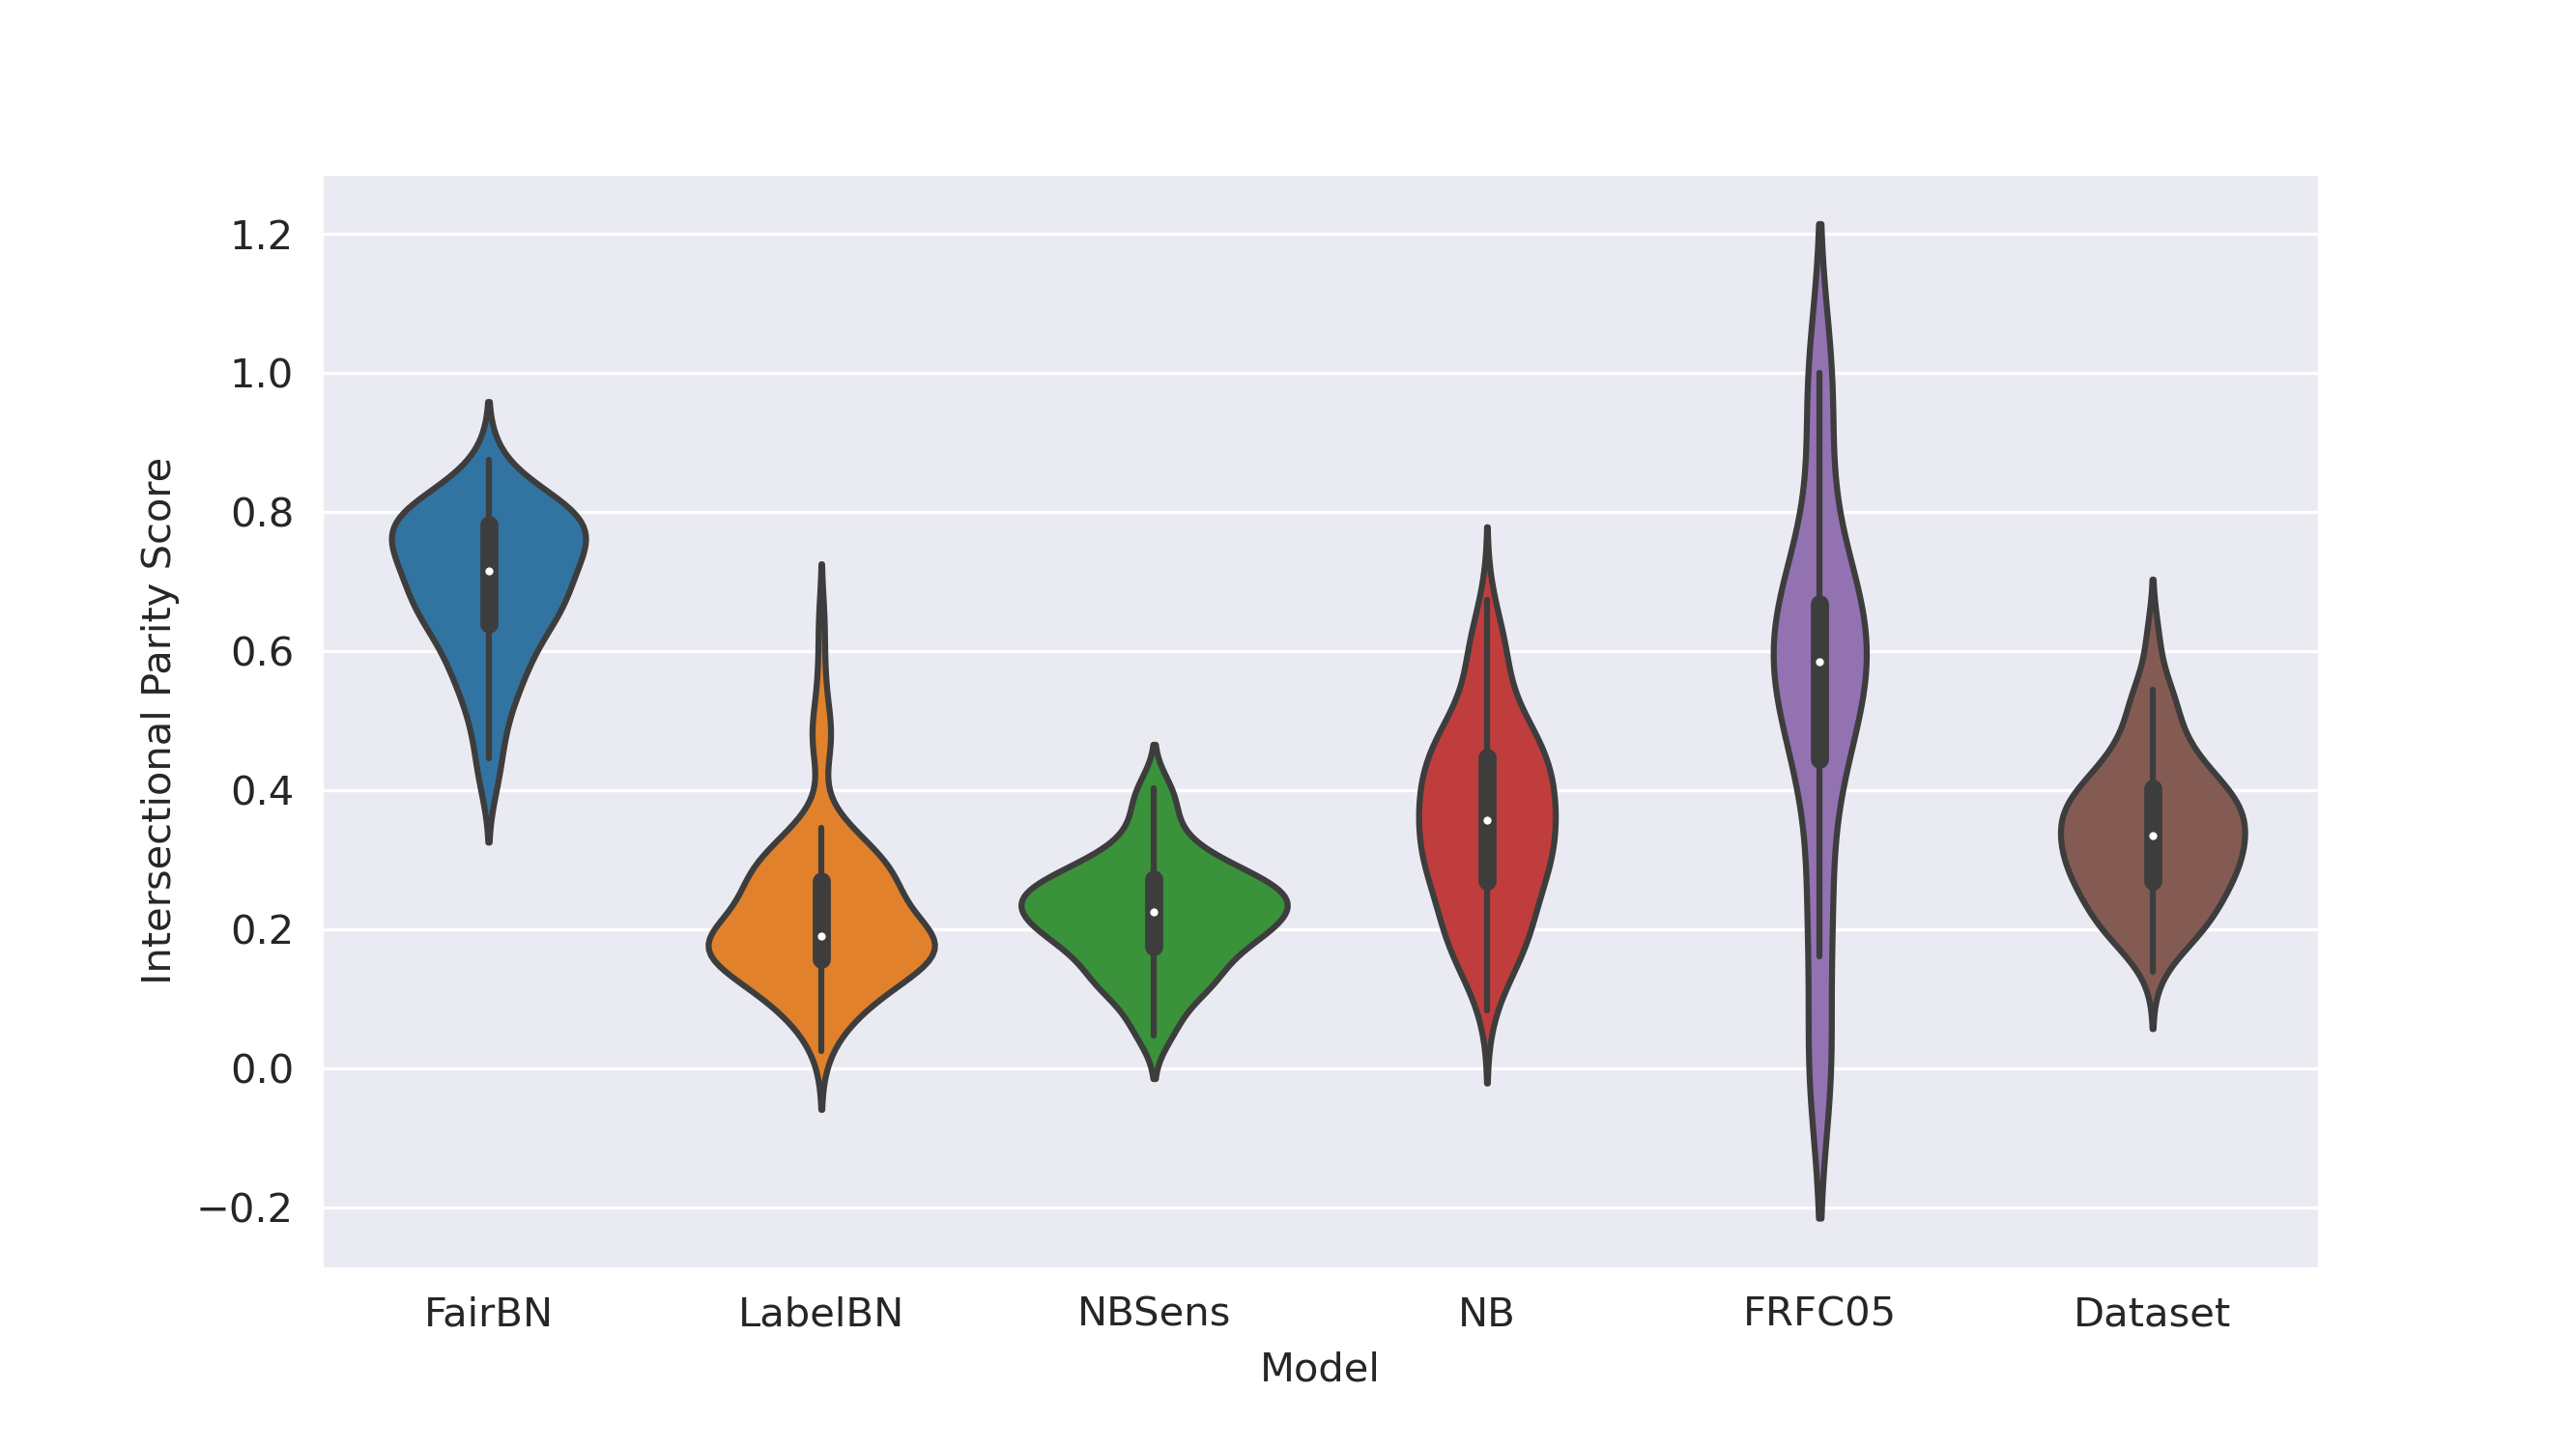
\includegraphics[width=\linewidth]{figures/intparscore-synthetic.png}
    \caption{Intersectional Parity Score of the different models on 100 synthetic datasets. Higher is better.}
    \label{fig:intpar}
\end{figure}

In terms of intersectional parity score, i.e. average demographic parity across all subgroups of sensitive attributes, we see that the fair bayesian network is able to consistently have more fair decisions. See figure~\ref{fig:intpar}. On average the mean parity score for the FairBN classifier is $0.70$ with the 5th percentile at $0.50$. For the fair random forest classifier these values are $0.54$ and $0.0$ respectively.
 
\subsubsection{AUC Gender}

\begin{figure}
    \centering
    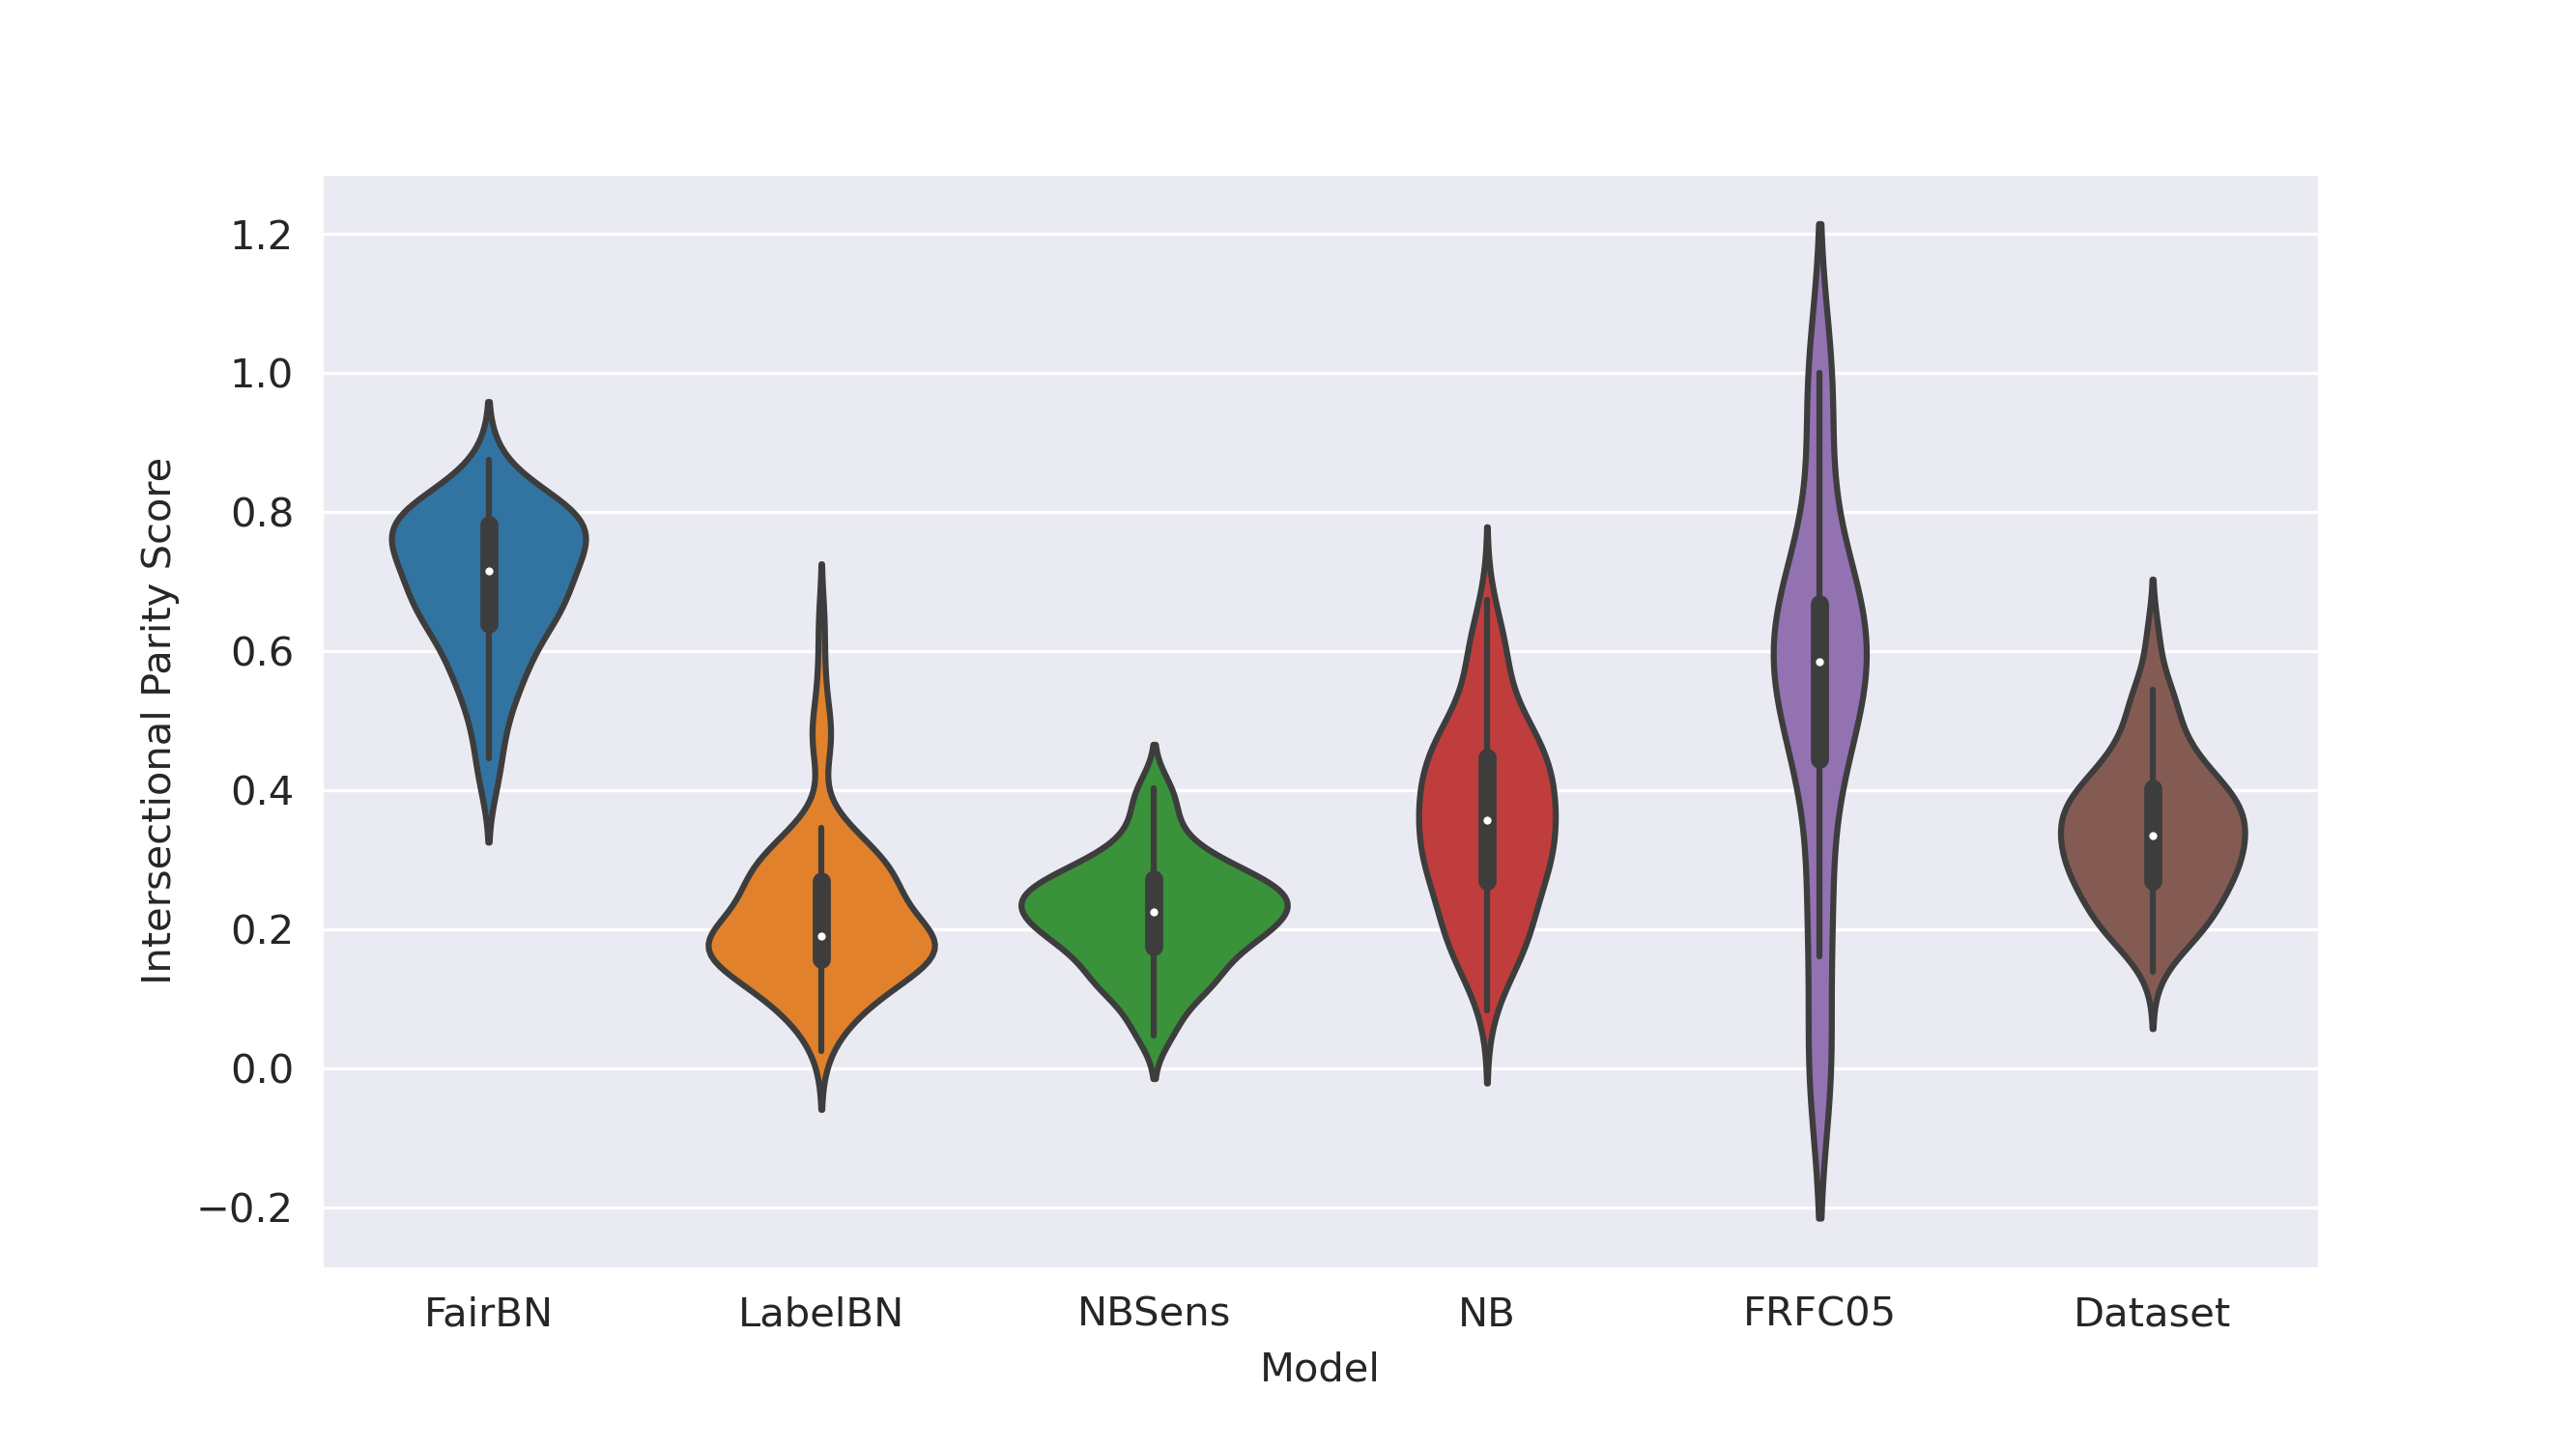
\includegraphics[width=\linewidth]{figures/intparscore-synthetic.png}
    \caption{AUC wrt Gender of the different models on 100 synthetic datasets. Lower is better.}
    \label{fig:aucgender}
\end{figure}

In the paper by \citet{Antonio:2021:arXiv} they propose use AUC wrt gender to evaluate splits which are more fair. Interestingly, while the fair random forest method is based on selecting splits that minimise the AUC wrt gender, the model fares quite similarly to the Naibe Bayes models and LabelBN. See figure~\ref{fig:aucgender} The AUC is even higher than what is inherent in the labels of the dataset itself and predictions are in this sense more discriminatory than what is present in the true labels. The only model to minimise AUC more than the inherent dataset labels is FairBN. FairBN has a mean AUC of $0.56$ and a 5th percentile of $0.51$. While for the fair random forest classifier, these values are $0.72$ and $0.51$ respectively.

\subsubsection{Kullback-Leibler Divergence}

\begin{figure}
    \centering
    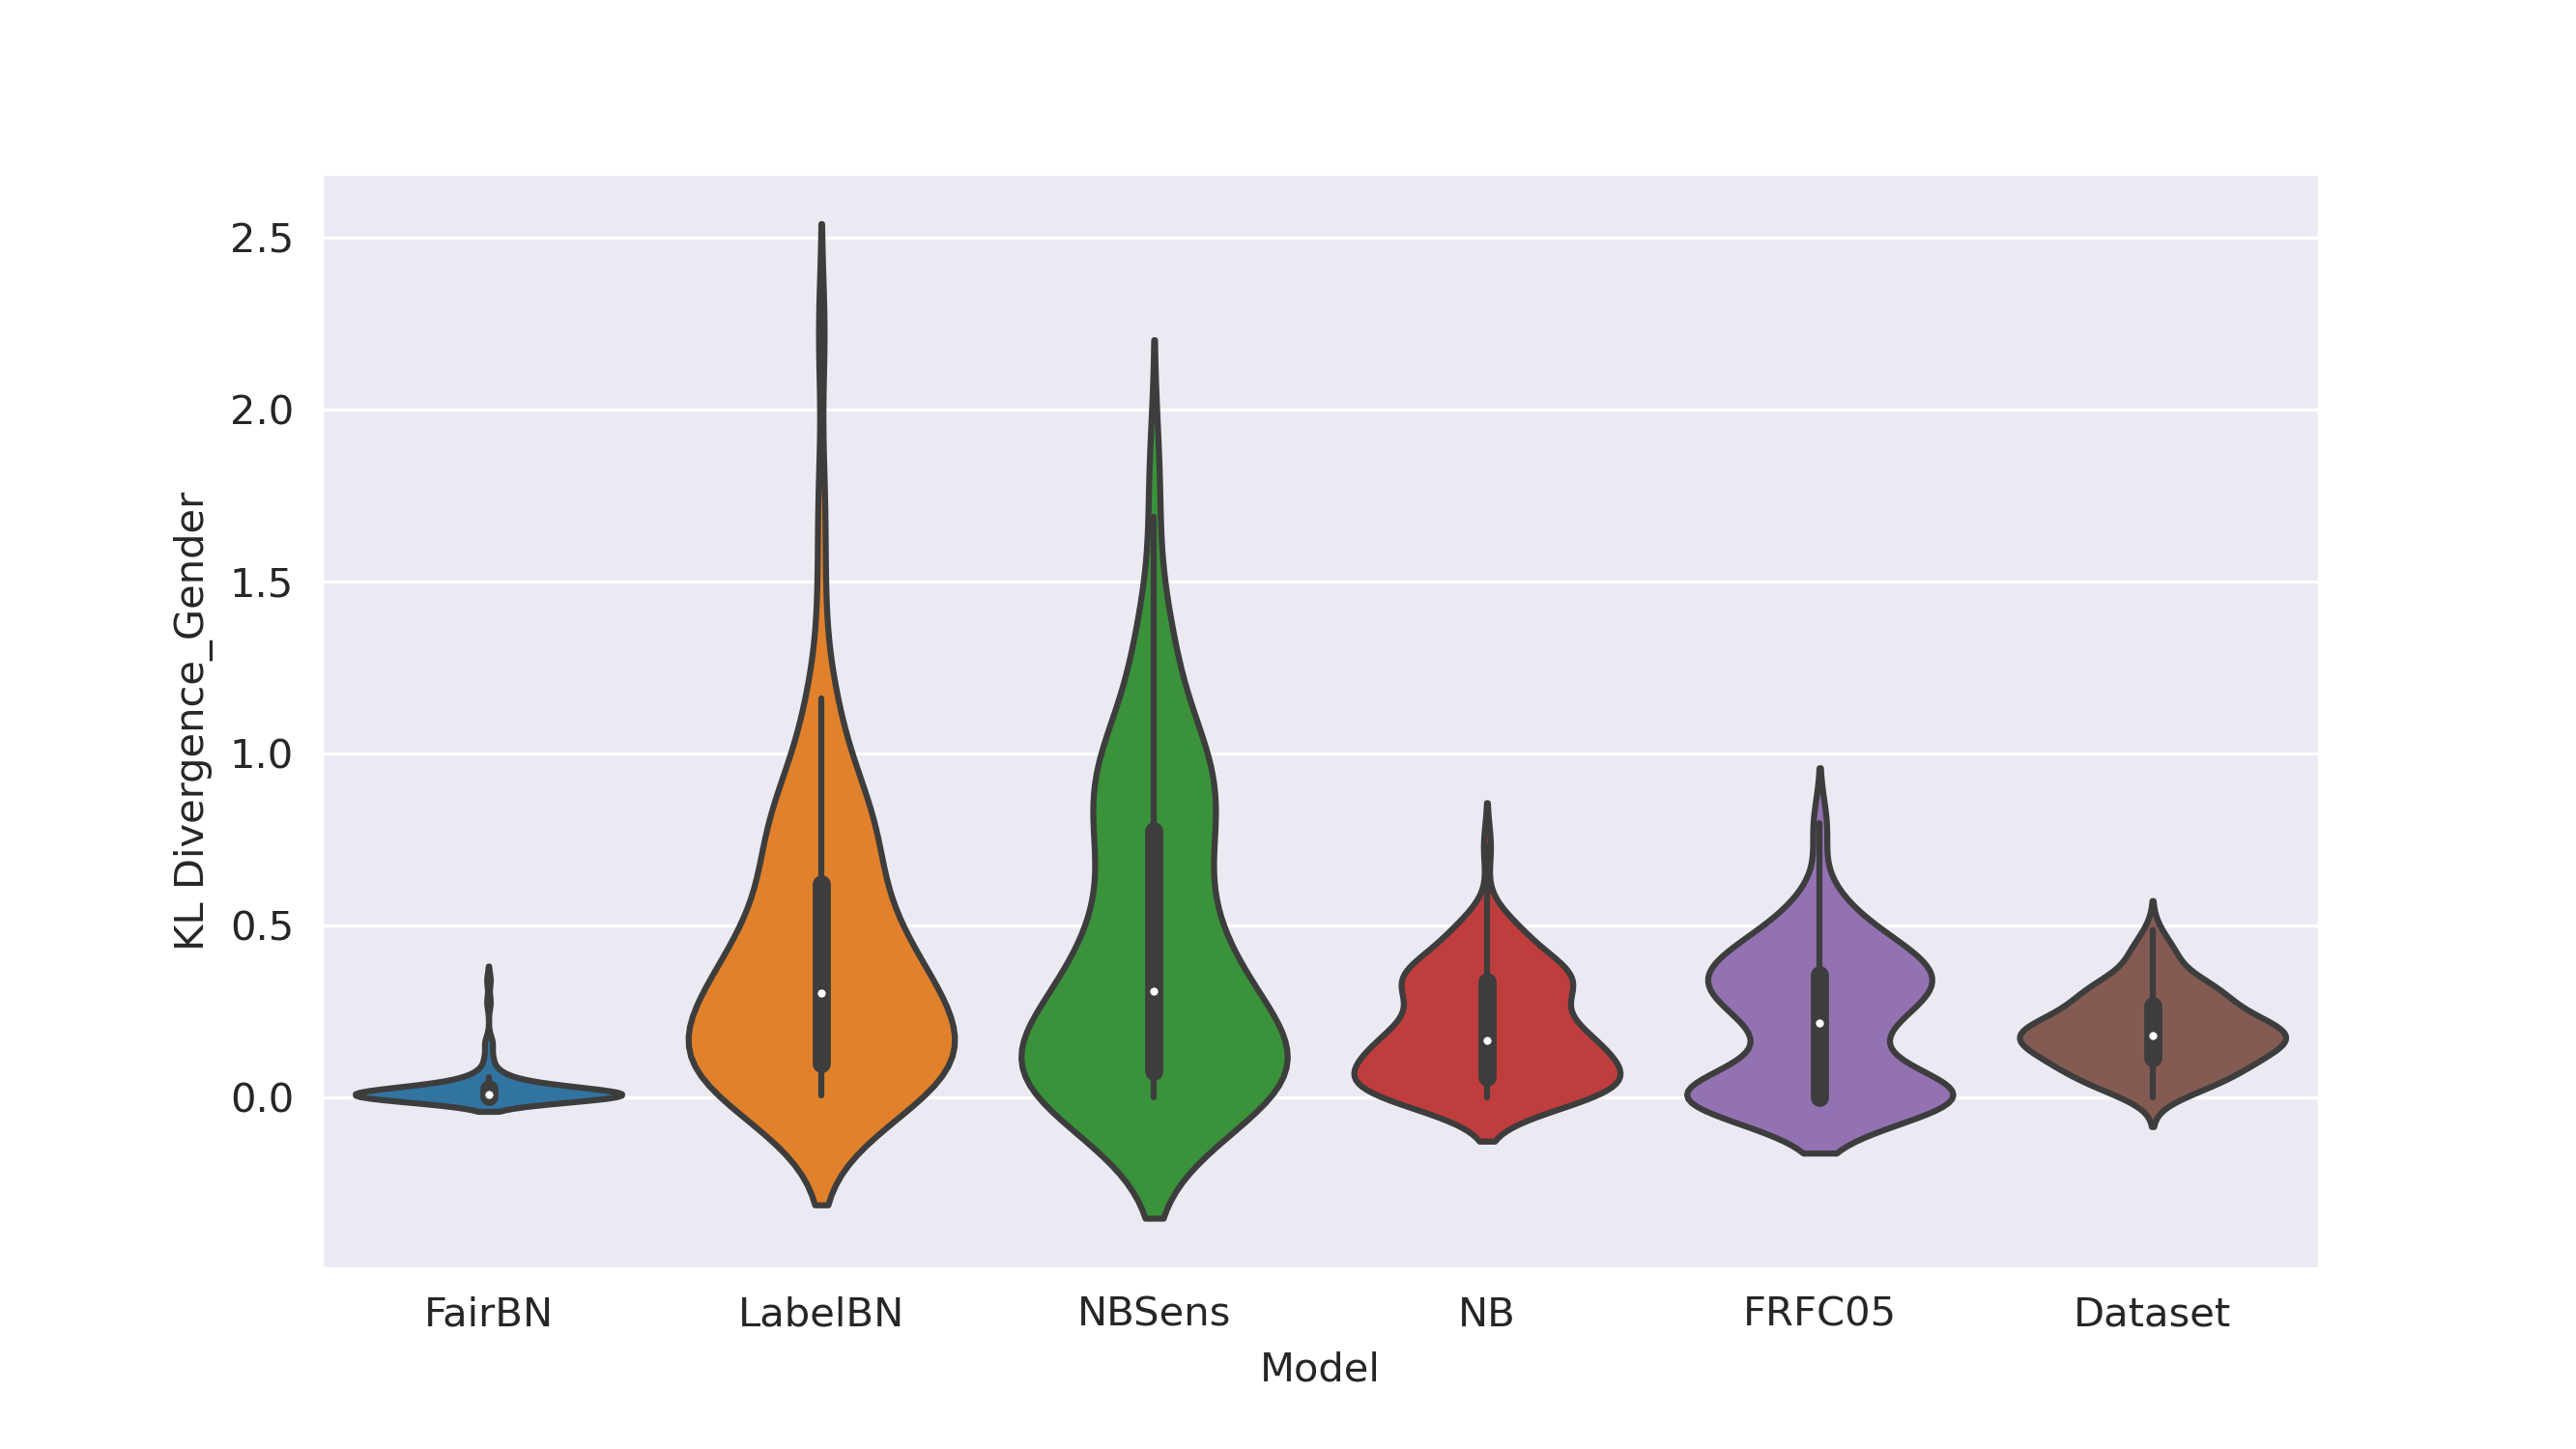
\includegraphics[width=\linewidth]{figures/kldg-synthetic.png}
    \caption{Kullback-Leibler Divergence of the different models on 100 synthetic datasets. Lower is better.}
    \label{fig:kldg-synthetic}
\end{figure}

Lastly, we evaluate the models in terms of Kullback-Leibler Divergence. Here we see a significant difference between the methods. See figure~\ref{fig:kldg-synthetic}The best performing model here is FairBN. With a 5th percentile value of $4.67 \times 10^{-5}$ and mean $0.025$. For the fair random forest classifier this is $0$ and $0.21$ respectively

\section{Interpretable Machine Learning}

Some of the models that we have trained are interpretable. These are the Naive Bayesian models and the Fair Bayesian Network. While we have implemented a fair random forest method, this is not immediately interpretable. Therefore, we will train decision trees on the data using ScikitLearn to see the decision behind the predictions as well as the importance of features. Additionally, an effort on trying to extract the feature importance in the random forests model.

\subsection{Interpreting Decision Trees}

According to \citet{Molnar:2020:Book} the interpretation of decision trees, while quite similar for all algorithms, differ by the kind og algorithm for building the tree is used. The interpretation described here is for the CART algorithm which is the one implemented by ScikitLearn \cite{Pedregosa:2011:JMLR}.

The interpretation of decision trees works as follows: Starting from the root node, you go to the next nodes and the edges tell you which subsets you are looking at. Once you reach the leaf node, the node tells you the predicted outcome. \cite{Molnar:2020:Book}

To calculate the feature importance. We calculate the reduction in the split. In our case, we have used entropy and information gain to evaluate splits which is defined as 

\begin{equation*}
    IG(T) = H(T) - \sum_{i = 1}^{2} \frac{n_i}{n} H(C_i)
\end{equation*}

Where $T$ is the node being split and $C_i$ is child node $i$. $H$ denotes shannon entropy introduced by \citet{Shannon:1948:BellSystTechJ}. Go through all the splits for which the feature was used and measure how much it has reduced the information gain. Scale all the sums to $1$, then you can calculate the share of a features importance as an percentage.

We will do this for the datasets that have been used in the previous experiments to uncover what attributes are used in the model prediction.

\subsection{Interpreting Fair Random Forest}



\subsection{Interpreting Naive Bayes}

As described in section~\ref{relatedwork:naivebayes}, the Naive Bayes classifier assumes that all features are mutually independent, conditioned on the class labels. We can therefore interpret the contributions of the different attributes through the conditional probabilities that the Naive Bayes classifier has learned \cite[p.~142]{Molnar:2020:Book}.

The way we have chosen to do this is like so: Assume that a feature $X_i$ in a dataset $\boldsymbol{X}$ is informative. Then we would expect that the likelihood on $X_i$ is very different given the class $Y$

\begin{equation*}
    P(X_i | Y = 0) \neq P(X_i | Y = 1)
\end{equation*}

In the case that $X_i$ is categorical with $k$ categories. We have a conditional dependency table on the form

\begin{equation*}
    \begin{bmatrix}
        P(X_0 | Y = 0) & P(X_0 | Y = 1) \\ 
        P(X_1 | Y = 0) & P(X_1 | Y = 1) \\
        \vdots & \vdots \\
        P(X_k | Y = 0) & P(X_k | Y = 0)
    \end{bmatrix}
\end{equation*}

Then we denote the first column $P = P(X_i | Y = 0)$ and the second column $Q = P(X_i | Y = 1)$. We assume that the more informative $X_i$ is as a feature, the difference in these distributions should increase. To calculate the feature weight we define the weight as 

\begin{equation*}
    D_{KL}(P||Q)
\end{equation*}

This should also be validated using permutation importance to compare the weights. Introduced by \citet[p.23-25]{Breiman:2021:MachLearn}. The algorithms used is shown below and is based on the one used by ScikitLearn \cite{Pedregosa:2011:JMLR}

\begin{algorithm}
    \caption{Permutation Importance Algorithm}
    \begin{algorithmic}
        \REQUIRE $C = $ Classifier, $D = $ Test Dataset. $K = $ No of permutations.
        \ENSURE $I = $ Dataset of importances.
        \STATE Compute reference score $S$ on the test dataset $D$.
        \FORALL{columns $i\in D$}
            \FOR{$j \in \{ 1, \dots, K \}$} 
                \STATE Permute (shuffle) column $D_{i}$ and denote the corrupted dataset $\Tilde{D}_{j}$
                \STATE Compute score $s_{ij}$ on test dataset $\Tilde{D}_{j}$
                \STATE Set $I_{ij} = S - s_{ij}$
            \ENDFOR
        \ENDFOR
        \RETURN $I$ 
    \end{algorithmic}
\end{algorithm}

This algorithm returns a dataset of importances as we want to see the distribution of importances for each feature.

\subsection{Interpreting Bayesian Networks}

